\documentclass[journal=jpcbfk,manuscript=article,layout=twocolumn]{achemso}
\usepackage{amsmath}
\usepackage{amssymb}
%\usepackage{widetext}
\usepackage{verbatim}
\usepackage{graphicx}
% \usepackage{multicol}
\usepackage[normalem]{ulem} % for strikethrough
\usepackage[obeyFinal]{easy-todo}
\usepackage{dutchcal}
\usepackage{xfrac}
\usepackage{footmisc}

\newcommand{\figurewidth}{.48\textwidth}
\renewcommand{\epsilon}{\varepsilon}
\newcommand{\dz}{\,\mathrm{d}z}
\graphicspath{{Figures/}}
\newcommand{\onlinecite}[1]{\hspace{-1 ex} \nocite{#1}\citenum{#1}}
\SectionNumbersOn
%\DeclareUnicodeCharacter{2009}{FIXME}

\author{Hanne S. Antila}
\affiliation{Department of Theory and Bio-Systems, Max Planck Institute of Colloids and Interfaces, 14424 Potsdam, Germany}

\author{Tiago Ferreira}
\affiliation{NMR Group --- Institute for Physics, Martin-Luther University Halle--Wittenberg, 06120 Halle (Saale), Germany}

\author{Matti Javanainen}
\affiliation{Add Matti to author list?}

\author{O. H. Samuli Ollila}
\affiliation{Institute of Biotechnology, University of Helsinki, 00014 Helsinki, Finland}

\author{Markus S. Miettinen}
\affiliation{Department of Theory and Bio-Systems, Max Planck Institute of Colloids and Interfaces, 14424 Potsdam, Germany}
\email{markus.miettinen@iki.fi}

%\title{Using open data to benchmark internal dynamics of phosphatidylcholine in molecular dynamics simulations}
\title{Using open data to rapidly bench\-mark bio\-molecular simulations: Phospholipid internal dynamics}
\begin{document}


\begin{abstract}
Molecular dynamics (MD) simulations are widely used to
    study the atomistic structure and dynamics of biomembranes. It
    remains unknown, however, how well the conformational dynamics
    observed in MD simulations correspond to those occurring in real
    life phospholipids. The accuracy of such time scales in MD can be
    assessed by comparing against the effective correlation times $\tau_\mathrm e$ of
    the C-H bonds measured in nuclear magnetic resonance experiments
    (J. Chem. Phys. 142 044905 (2015)).

    Here, we extend this previous analysis by considering carefully the error estimation of MD-determined $\tau_\mathrm e$,
    and analyze the conformational dynamics of phospholipids as
    produced by several commonly used MD models (force fields).
    None of the tested force fields reproduced all the effective
    correlation times within experimental error, much like they do
    not provide accurate conformational ensemble (J. Phys. Chem. B 119 15075 (2015)). However, the
    dynamics observed in CHARMM36 and Slipids were more realistic
    than those seen in the Amber Lipid14, OPLS-based MacRog, and
    GROMOS-based Berger force fields, where dynamics of the glycerol backbone was unrealistically slow.
\end{abstract}

\section{Introduction}
Ever since the conception of Protein Data Bank (PDB)~\cite{nnb1971,wwPDB2019} and GenBank~\cite{jordan1982,sayers2020},
open access to standardised and searchable pools of experimental data has
%shaped the state of the art of 
revolutionized
research in life sciences.
The databanks~\cite{Gaber:2019a}, constantly growing and improving in fidelity~\cite{hobohm1992,levitt2007,meszaros2019}
%as well as identifying~\cite{hobohm1992,levitt2007} and filling~\cite{meszaros2019} gaps in the databanks themselves
due to collaborative effort, enable scientific progress that is well beyond the resources of one single research group, giving rise to entirely new ways of doing science in the form of bio- and cheminformatics, and enabling data-driven development of 
characterisation techniques~\cite{burley2018}, %(such as molecular replacement~\cite{rossmann62} in macromolecular x-ray crystallography and 3D electron microscopy) 
drugs~\cite{kirchmair08}, and materials~\cite{huang2016}.
%
%Today these data banks are regarded irreplaceable core resources. The cost of reproducing all the data in PDB has been estimated to be X and destruction of the databank would lead to a near complete halt both academic and commercial research.
%
%Much of the development of the PDB and other biomolecular databanks into the core resources they are today has been fueled by
%In addition to experimental results, the push from %scientific journals and
%funders towards
The idea of public availability and conservation of data has recently extended also to molecular dynamics (MD) simulation trajectories of biomolecules, and discussion on how and by whom these databases for dynamic information would be set up is currently active~\cite{Hildebrand:2019a,Abraham:2019a,Gygli:2020a,Abriata:2020a,Hospital:2020a}.
%
\todo{Mention GPCRmd~\cite{Rodriguez-Espigares:2019a}? SAMULI: I think yes.}
%Notably,

Since 2013 the NRMlipids Project (\url{ nmrlipids.blogspot.fi}) has
promoted an open collaboration approach,
where the whole research process, from the initial ideas and discussions to
the analysis methods, data and publications, are publicly available all the time \cite{botan15}.
While the main focus of the NMRlipids Project has been in conformational ensembles
of lipid headgroups and ion binding to lipid membranes \cite{botan15,catte16,antila19},
it has also accumulated a collection 
%such a databank~\cite{Miettinen:2019c} for
of atomistic MD simulations of lipid membranes containing hundreds of trajectories ({\tt zenodo.org/communities/nmrlipids}).
These data are also partially indexed at \url{www.nmrlipids.fi}.
%\todo{HA: bit of a conceptual jump hereto the next paragrap, added the sentence below to soften it
%SAMULI: I have proposed modifications here which hopefully help.}
Such databanks are particularly relevant for disordered molecules, such as %Our system of interest,
biological lipids composing cellular membranes, which cannot be descibed by coordinates of single structure in contrast to
folded proteins or DNA strands.
%, in their biologically relevant state as the core components of the cell's membranes, are intrinsically unstructured.
Realistic MD simulations can provide conformational ensemble and dynamics of such molecules as well as
enable studies of their biological functions in complex biomolecules assemblies.
However, current MD simulation force fields largely fail to capture conformational ensembles of lipid headgroups and
disordered proteins \cite{botan15,antila19,??}.
Therefore, the quality of MD simulations in databanks and other applications must be carefully assessed against
experimental data.
For lipid bilayers, such evaluation is possible against NMR and scattering data \cite{ollila16}.
%To properly describe such molecules, a whole ensemble of conformations as well as the dynamics linking them is needed.
%To obtain such description, MD simulations of lamellar phospholipid bilayer systems are widely 
%%Although biological membranes are complex mixtures of multiple lipid types as well as other molecules,
%%bilayer with one or few lipid types serve as an important model system, that have been successfully used
%used~\cite{lyubartsev11,chau07,ferreira13,botan15, ferreira15,miettinen19,XXX}, and
%hold vast potential to decipher, e.g., molecular mechanisms behind anesthetics~\cite{chau07,XXX}, the effect of cholesterol on membrane structure~\cite{XXX,ferreira13}, and the functioning of membrane proteins~\cite{lindahl08} \todo{add more references?}.

Here, we demonstrate how publicly available set of MD simulation data can be utilized to
rapidly evaluate how fast individual lipid molecules sample their conformational ensemble
against experimental data in different force fields with unprecedented extent. 
%Using this freely available resource we demonstrate here, for the first time, the viability of creating new scientific knowledge solely through analysis of pre-existing, open access MD simulation data.
MD simulations with correct lipid dynamics are desired, for example, for the interpretation of
NMR or other experiments detecting molecular dynamics and to understand dynamics of biological processes where
lipid deformations have rate limiting role such as membrane fusion \cite{??}.
In addition, 
%However, to be truly useful MD should
%%The significance for investigating the conformational dynamics of lipids in bilayer simulations is two-fold.
%give the right 1) equilibrium statistics and 2) dynamics.
%To extract reliable statistics,
information on dynamics is crucial to assess if simulations have converged.%:
%The conformations sampled have to represent the equilibrium distribution with enough transitions between states. Indeed, for lipids even 500\,ns simulations might be insufficient~\cite{vogel12,ferreira15}.
%Simulations of a single (1,2-dioleoyl-sn-glycero-3-phosphocholine) DOPC lipid using the CHARMM32b2 force field indicated that the conformations sampled do not replicate the equilibrium distribution even after 500 ns~\cite{vogel12}; also, the C--H bond dynamics of the Berger model was shown~\cite{ferreira15} to be too slow at the glycerol region of 1-palmitoyl-2-oleoylphosphatidylcholine (POPC) compared to correlation times extracted from NMR experiments.
%
%Along with equilibrium statistics, the ability of MD to reproduce the bilayer dynamics is equally crucial for an accurate picture of membrane function. %in addition to equilibrium measurements are. 
%The correct relative abundance of different dynamical processes is needed for reliable interpretation of pathways leading to, e.g., membrane deformation~\cite{chernomordik08} and lipid-induced conformational~\cite{gibson93,phillips09} changes of membrane proteins. Notably, the availability of such a realistic MD model could greatly guide both the configuration and the interpretation of NMR experiments used to extract dynamical information from lipid assemblies.

%%We will check the lipid dynamics in existing MD models using the existing NMRlipids databank.
%%
%%More specifically,
%By analyzing a wide set of publicly available phosphatidylcholine (PC) lipid bilayer MD trajectories, we test whether different MD models (force fields) reproduce the experimentally observed internal dynamics of PC lipids, and investigate if the dynamics of various models share common features. Such features can be used to draw general conclusions on the system, to avoid potential pitfalls in future simulations of bilayers, and to suggest future directions for experimental research.  In addition to simulations of one component bilayers under standard conditions, we study the effects of varying hydration, cholesterol content, and NaCl concentration.



%Our choice for the system of interest is inspired by the importance of phospholipids %not only
%as the building blocks of cell membranes.
%but also as emerging candidates for micro- and nanotechnology, such as the use of liposomes as microcapsules in targeted drug delivery~\cite{sercombe15}. These molecules consist of a hydrophilic phosphate head group, which is connected to two hydrophobic fatty acid tails via a glycerol backbone. The ability of lipids to self assemble into bilayer membrane (and other) configurations is a direct consequence of this dual nature.

%We believe that
Our comprehensive comparison of dynamics between different MD models for phosphatidylcholine lipids
with varying biologically relevant compositions and conditions paves the way for the development of more realistic lipid force fields.
%where both pure bilayers and the model response to changing conditions and composition is explored.
%The study is conducted using pre-existing, publicly available simulation trajectories to demonstrate the power of open,
%well documented MD data in creating new knowledge at a lowered computational cost and high potential for automation.  
Furthermore, the analysis of extensive set of data from different models shed light on the complex
dynamics lipid in their biological relevant disordered state.
Our results demonstrate the power of publicly available simulation trajectories  %open, well documented MD data
in creating new knowledge at a lowered computational cost and high potential for automation.  
%the pre-existing, 
We believe that our work paves the way for novel applications of publicly
available MD simulations databanks, as well as demonstrates their usefullness not only for lipid bilayers
but also for other biomolecular systems.

%we intentionally restrict ourselves to re-use existing, publicly available simulation trajectories. This is to demonstrate the power of open, well documented data in creating new knowledge at a lowered cost. The main source of data was the collection of lipid bilayer simulations originating from the NMRlipids project~\cite{botan15,catte16}

%Both the  have been traditionally assessed based on the spin-lattice relaxation rates $R_{1}$ (or the corresponding $T_{1}$ times), available through NMR measurements. At best, the simulation can be combined with the NMR experiments to provide an interpretation of the molecular motion~\cite{pastor88,klauda08,klauda08II}.  


%Here, we use the effective correlation time to present the first comprehensive comparison of dynamics of 1-palmitoyl-2-oleoylphosphatidylcholine (POPC) in different MD models. We not only investigate the pure bilayers in room temperature but also explore the effect of cholesterol content, hydration and monovalent salt to see whether the model dynamics correctly responds to the change in conditions. An MD model fulfilling these requirements can provide a reliable tool to study, e.g., membrane remodeling, or to interpret the experimental spin relaxation rates by connecting them to the underlying dynamical processes. 

%Within this study, we intentionally restrict ourselves to re-use existing, publicly available simulation trajectories. This is to demonstrate the power of open, well documented data in creating new knowledge at a lowered cost. The main source of data was the collection of lipid bilayer simulations originating from the NMRlipids project~\cite{botan15,catte16}. \todo{Start the intro with this, i.e., open data?}


\section{Methods}
\subsection{Evaluation of conformational dynamics of lipids against NMR data}\label{sec:theory}
We analyze lipid dynamics based on two quantities available from published $^{13}$C-NMR experiments:~\cite{ferreira15,pham15,Volke:1995a}
The effective C--H bond correlation time $\tau_\mathrm{e}$ and
the spin-lattice relaxation rate $R_{1}$,
both %experimentally available through NMR measurements, and
directly quantifiable from atomistic MD simulations.
The
$\tau_\mathrm e$ are effectively an average over all the time scales relevant for the lipid internal dynamics,
and respond intuitively to changes in these: 
%Most importantly, i
Increasing $\tau_\mathrm{e}$ always signals some type of slowdown in the C--H bond dynamics. %, making the interpretation less ambiguous than for $R_1$, where slowdown in the dynamics can lead to either an increase or a decrease of $R_{1}$ value
\cite{ferreira15}
%
The $R_{1}$ rates (or the corresponding $T_{1}$ times) have been traditionally used to assess both the conformational dynamics of lipids in experiments~\cite{feller02,eldho03,wohlert06,klauda08,leftin11} and the dynamics produced by MD models in simulations~\cite{feller02,wohlert06,klauda08,klauda08II}.
In contrast to $\tau_\mathrm e$, the $R_1$ are sensitive to processes within a rather narrow time scale window set by the magnet frequency, and changes in $R_1$ are not intuitively related to changes in process speeds: A decrease in $R_1$ tells that the amount of processes in the sensitive time window decreases, but not if the corresponding processes become faster or slower.
%However, relying on $R_{1}$ only has several drawbacks. \todo{Do all flavors ($^{31}$P, $^{13}$C,\ldots) have the same problem?} It builds on an underlying rotation-diffusion model, its sensitivity is typically limited to C--H bond reorientation with time scales $\sim$1-10 ns, and
%Therefore, measurements at several temperatures and magnetic field strengths are required to fully characterize the dynamics. %To address these deficiencies, two of us introduced a procedure~\cite{ferreira15} for quantifying the effective C--H correlation times ($\tau_\mathrm{e}$)---a model free quantity that encompasses conformational dynamics with time scales up to hundreds of nanoseconds---from bilayer systems.

$^{13}$C NMR experiments investigating lipid conformational dynamics take advantage of the fact that the relaxation of $^{13}$C magnetization dominantly happens via the dipolar coupling of the carbon with the magnetic moments of the protons bound to it, with the symmetry axis of the interaction aligning with the C--H bond. The spectral density depicting the $^{13}$C relaxation rates (at frequency $\omega$) is expressed as
\begin{equation}
j{(\omega)}=2\int_{0}^{\infty}\cos(\omega\tau)g(\tau)\mathrm d\tau ,
\end{equation}
which is the Fourier transformation of the C--H bond second order autocorrelation function at time $\tau$
\begin{equation}
\label{eq:BCF}
g(\tau)=\langle P_{2}\left(\vec{\mu}(t)\cdot \vec{\mu}(t+\tau)\right)\rangle ,
\end{equation}
where $\vec{\mu}(t)$ is the unit vector in the direction of the C--H bond at time $t$ and $P_{2}$ is the second order Legendre polynomial. The angular brackets depict averaging over time. The autocorrelation function can be expressed as the product of two functions
\begin{equation}
g(\tau)=g_{\mathrm{f}}(\tau)g_{\mathrm{s}}(\tau) ,
\end{equation} 
where $g_{\mathrm{f}}(\tau)$ characterizes fast decays owing to, for example, the molecular  rotations, and $g_{\mathrm{s}}(\tau)$ describes slow decays that originate from, e.g., lipid diffusion. The two components, along with the oscillation due to magic angle spinning at the $\sim$kHz region, are depicted in Fig.~\ref{fig:schem_teff}. Correlation time of 4.2 ms has been estimated for multilamellar POPC samples at 300 K for the slow modes, whereas  in liquid crystalline lipid bilayers the faster $g_{\mathrm{f}}(\tau)$ decays to a plateau value $S^{2}_{\rm{CH}}$ within a few hundred nanoseconds~\cite{ferreira15}. The C--H bond order parameters
\begin{equation}
\label{eq:OP}
S_{\rm{CH}}=\frac{1}{2}\langle 3\cos^{2}\theta(t)-1\rangle ,
\end{equation}
where $\theta(t)$ is the angle between the bond and the bilayer normal, are measured in NMR experiments from this plateau. As $S_{\rm{CH}}$ describes the conformational ensemble of the molecule, the fast-decaying component of the rotational correlation function intuitively depicts the time needed to sample these conformations. The characteristic time can be quantified via the effective correlation time
\begin{equation}
\label{eq:teff}
\tau_\mathrm{e}=\int_{0}^{\infty}\frac{g_{\mathrm{f}}(\tau)-S^{2}_{\rm{CH}}}{1-S^2_{\mathrm{CH}}}\mathrm d\tau.
\end{equation}
The integrand can be viewed as a reduced and normalized correlation function
\begin{equation}
\label{eq:nBCF}
g'_{\mathrm{f}}(\tau)=\frac{g_{\mathrm{f}}(\tau)-S^{2}_{\rm{CH}}}{1-S^2_{\mathrm{CH}}}.
\end{equation}
That is, $\tau_\mathrm e$ is defined as the area under $g'_{\mathrm{f}}(\tau)$, as
graphically depicted in Fig.~\ref{fig:schem_teff}b.
\todo{Maybe also add 1C that explicitly shows $g'_{\mathrm{f}}$?}
It is easily seen that in the presence of more long-lived correlations $\tau_\mathrm{e}$ grows, signaling that more time is needed for full conformational sampling.  

\begin{figure}[t]
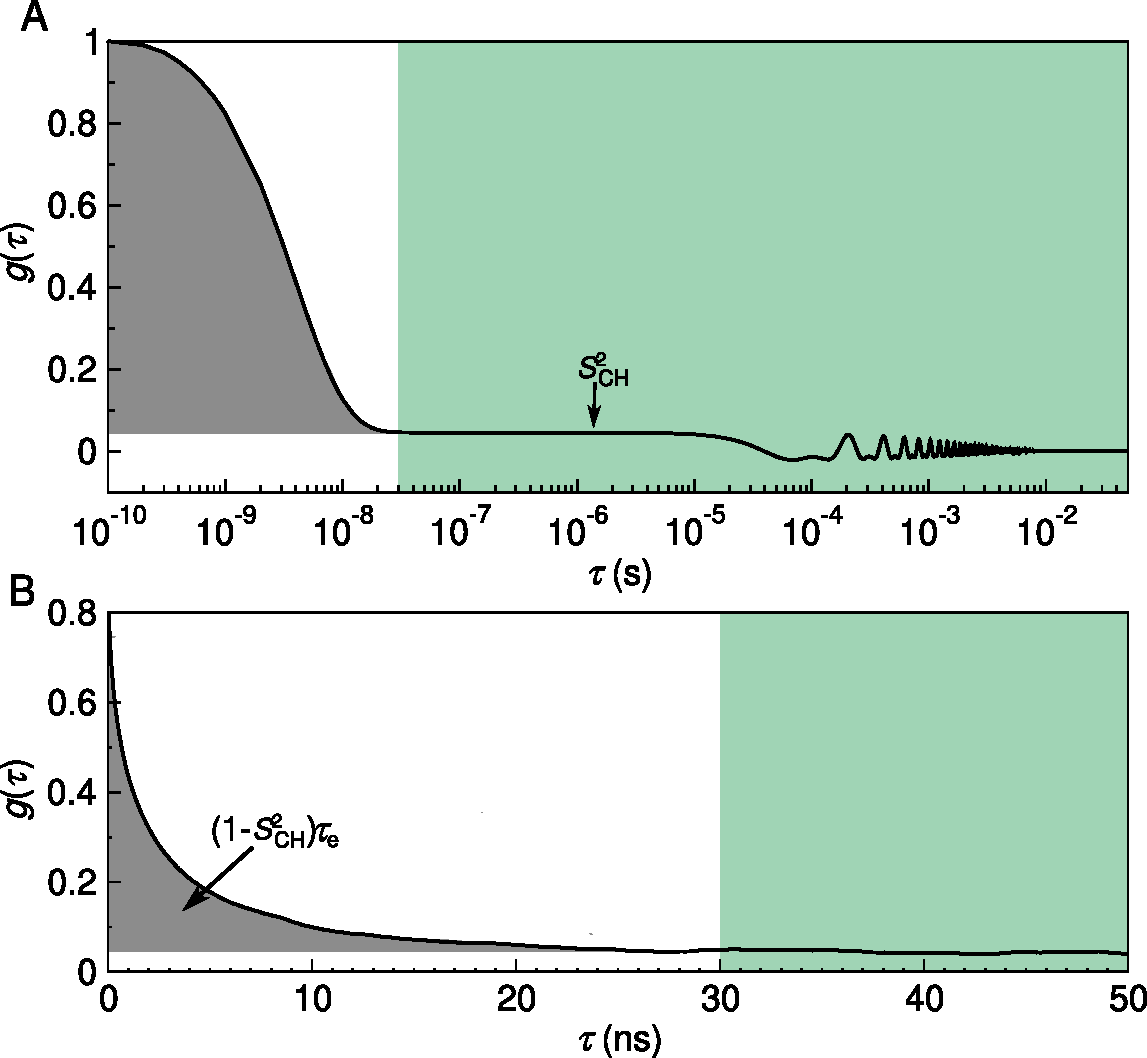
\includegraphics[scale=0.45]{./figures/gfun_draft.pdf} 
\caption{The autocorrelation function $g(\tau)$ a) The fast mode (white background) and the slow mode (shaded green) of the correlation function along with the oscillation owing to magic angle spinning. The fast mode decays to a plateau quantifying the $S_{\mathrm{CH}}$ while the slow mode gives the final descent to zero. b) Illustration of typical C--H bond autocorrelation function obtained from a MD simulation. The gray area under the curve gives a way of quantifying the $\tau_\mathrm{e}$. }
\label{fig:schem_teff}

\end{figure} 


The spin-lattice relaxation rate $R_1$ defines the time-scale on which $^{13}$C longitudal magnetization equilibrates. It is defined as  
\begin{align}
\label{eq:R1}
\begin{split}
R_{1}=&\frac{d^2_{\mathrm{CH}}N_{\mathrm{H}}}{20}\left[j(\omega_{\mathrm{H}}-\omega_{\mathrm{C}})\right. \\
&\left.+3j(\omega_{\mathrm{C}})+6j(\omega_{\mathrm{H}}+\omega_{\mathrm{C}})\right] ,
\end{split}
\end{align}
where $N_{\mathrm{H}}$ is the number of bound hydrogens, $\omega_{\mathrm{H}}$ and $\omega_{\mathrm{C}}$ are the Larmor frequencies for $^{1}$H and $^{13}$C, and $d_{\mathrm{CH}}$ is the rigid dipolar coupling constant. For the methylene bond, $d_{\mathrm{CH}}/2\pi$ approximately equals to -22~kHz.
\todo{why there is a minus sign above?}

The dependency of $R_{1}$ on the spectral densities $j$ at the Larmor frequencies means that the $R_{1}$ value depicts the relative amounts of relaxation processes with time-scales near the inverses of these frequencies. Since the Larmor frequencies depend on the field strength used in the NMR measurements, this typically makes $R_{1}$ sensitive to $\sim$1--10~ns time-scales. Importantly, a change in $R_{1}$ thus indicates a difference in the relative amounts of processes within the detection window, and therefore does not give information on the modulation of the total sampling rate.  


\begin{comment}
 The dipolar coupling constant $d_{\mathrm{CH}}$ is defined as

\begin{equation}
d_{\mathrm{CH}}=\frac{\hslash\gamma_{\mathrm{H}}\gamma_{\mathrm{C}}\mu_{0}}{4\pi\langle r^{3}_{\mathrm{CH}} \rangle} ,
\end{equation}

where $\hslash$ is the reduced Planck constant, $\gamma_{\mathrm{C}}$ and $\gamma_{\mathrm{H}}$ are the gyromagnetic constants for $^{1}H$ and $^{13}C$, $\mu_{0}$ is the vacuum permeability, and $\langle r^{3}_{\mathrm{CH}}\rangle$ denotes the average cubic length of the C-H bond.
\end{comment}

\subsection{Experimental data acquisition and analysis}
%
All the experimental quantities were collected from the literature \todo{Except are they, or mostly from Tiago and re-analysed from raw data?} sources referred at the respective figures \todo{How to refer to experimental data from Tiago?}.   

\subsection{Simulational data acquisition and analysis}
%
The simulation trajectories used in this work were collected from the Zenodo repository (\url{zenodo.org}) with majority of the data originating from the NMRlipids Project~\cite{botan15,catte16} (\url{nmrlipids.blogspot.fi}).
Table~\ref{tab:standr} details, with references to the trajectory files, the simulations of pure POPC bilayers at/near room temperature and at full hydration, whereas
Table~\ref{tab:chol} lists simulations including cholesterol;
Table~\ref{tab:hydr} simulations with varying hydration; and
Table~\ref{tab:salt} at increasing NaCl concentration.
Additional computational details for each of the simulations are available at the cited Zenodo entry.

\begin{table}[t!]
\caption{Analyzed simulations of POPC lipid bilayers at standard conditions.}
\begin{minipage}[t]{\columnwidth}
\resizebox{\columnwidth}{!}{
\begin{tabular}{lrrrrc}
%\hline
force field  &
$N_{\rm l}$\footnote{Number of POPC molecules.} &
$N_{\rm w}$\footnote{Number of water molecules.}  &
$T$\footnote{Simulation temperature.}(K) &
$t_{{\rm anal}}$\footnote{Trajectory length used for analysis.}(ns) &
files\footnote{Reference for the openly available simulation files.} \tabularnewline
\hline 
%Berger-POPC-07~\cite{ollila07a}
%	& 128 & 7290 & 298 & 50  & {[}\!\!\citenum{bergerFILESpopc}{]} \tabularnewline[1.0ex]
Berger-X~\cite{findrightffref}
	& 256 & 10240 & 300 & 300  & {[}\!\!\citenum{bergerFILESpopcT300}{]} \tabularnewline[1.0ex]	
CHARMM36~\cite{klauda10}
	& 256 & 8704 & 300 & 300 & {[}\!\!\citenum{charmm36filesT300}{]} \tabularnewline
%CHARMM36~\cite{klauda10}
%	& 34 & 1020 & 300 & 140 & {[}\!\!\citenum{charmm36filesHA}{]}\tabularnewline[1.0ex]
%MacRog~\cite{kulig15} 
%	&  128  & 6400 & 310 & 200  & {[}\!\!\citenum{macrogCHOLfiles}{]}\tabularnewline[1.0ex]
MacRog~\cite{kulig15} 
	&  128  & 5120 & 300 & 500  & {[}\!\!\citenum{macrogfilesT300}{]}\tabularnewline[1.0ex]
Lipid14 \cite{dickson14}
	& 72 & 2234 & 303 & 50 & {[}\!\!\citenum{lipid14files}{]}\tabularnewline[1.0ex]
Slipids~\cite{jambeck12b}
	& 200 & 9000 & 310 & 500  & {[}\!\!\citenum{slipidsFILESpopcchol}{]}\tabularnewline[1.0ex]
ECC~\cite{melcr18}
	& 128 & 6400 & 300 & 300  & {[}\!\!\citenum{eccFILESpopc}{]}\tabularnewline
\end{tabular}
}
\end{minipage}
\label{tab:standr}
\end{table}

\begin{table}[]
\caption{Analyzed simulations of cholesterol-containing POPC bilayers.}
\begin{minipage}[t]{\columnwidth}
\resizebox{\columnwidth}{!} {
\begin{tabular}{lrrrrrrc}
%\hline
force field POPC/cholesterol &
$c_{{\rm chol}}$\footnote{Bilayer cholesterol content (mol \%).}  &
$N_{\rm chol}$\footnote{Number of cholesterol molecules.}  &
$N_{\rm l}$\footnote{Number of POPC molecules.} &
$N_{\rm w}$\footnote{Number of water molecules.}  &
$T$\footnote{Simulation temperature.}(K) &
$t_{{\rm anal}}$\footnote{Trajectory length used for analysis.}(ns) &
files\footnote{Reference for the openly available simulation files.} 
\tabularnewline
\hline 
Berger-POPC-07~\cite{ollila07a}
	& 0\%	& 0	& 128	& 7290  & 298  & 50 & {[}\!\!\citenum{bergerFILESpopc}{]} \tabularnewline
/H\"{o}ltje-CHOL-13~\cite{holtje01,ferreira13} 
	& 50\%	& 64	& 64		& 10314  & 298  & 50  & {[}\!\!\citenum{bergerFILESpopc50chol}{]} \tabularnewline[1.0ex]
CHARMM36~\cite{klauda10} 
	& 0\%	& 0 	& 128 	& 5120  & 303  & 140  & {[}\!\!\citenum{charmm36files}{]} \tabularnewline
/CHARMM36~\cite{lim12} 
 	& 50\%	& 80	& 80		& 4496  & 303  & 200  & {[}\!\!\citenum{charmm36files50perCHOL}{]} \tabularnewline[1.0ex]
MacRog~\cite{kulig15}
	& 0\%	& 0	& 128	& 6400  & 310  & 500  & {[}\!\!\citenum{macrogCHOLfiles}{]} \tabularnewline
/MacRog~\cite{kulig15}
 	& 50\%	& 64	& 64		& 6400  & 310  & 500  & {[}\!\!\citenum{macrogCHOLfiles}{]} \tabularnewline[1.0ex]
Slipids~\cite{jambeck12b}
	& 0\%	& 0	& 200	& 9000 & 310 & 500  & {[}\!\!\citenum{slipidsFILESpopcchol}{]} \tabularnewline
/Slipids~\cite{jambeck13chol}
 	& 50\%	&200& 200	& 18000 & 310 & 500 & {[}\!\!\citenum{slipidsFILESpopcchol}{]}\tabularnewline
\end{tabular}
}
\end{minipage}
\label{tab:chol}
\end{table}

\begin{table}[]
\caption{Analyzed simulations of lipid bilayers under varying hydration level.}
\begin{minipage}[t]{\columnwidth}
\resizebox{\columnwidth}{!} {
\begin{tabular}{llrrrrrc}
%\hline
force field  &
lipid  &
$n_{{\mathrm w\!}_{/\mathrm l}}$\footnote{Water/lipid molar ratio.}  &
$N_{\rm l}$\footnote{Number of lipid molecules.}  &
$N_{\rm w}$\footnote{Number of water molecules.} &
$T$\footnote{Simulation temperature.}(K)  &
$t_{{\rm anal}}$\footnote{Trajectory length used for analysis.}(ns) &
files\footnote{Reference for the openly available simulation files.} \tabularnewline
\hline 
Berger-POPC-07~\cite{ollila07a} 
	& POPC  & 57  & 128  & 7290  & 298  & 50 & {[}\!\!\citenum{bergerFILESpopc}{]} \tabularnewline
	& POPC  & 7  & 128  & 896  & 298  & 60  & {[}\!\!\citenum{bergerDEHYDfiles}{]} \tabularnewline	
Berger-X~\cite{findrightffref}
	& POPC & 40 & 256 & 10240 & 300 & 300  & {[}\!\!\citenum{bergerFILESpopcT300}{]} \tabularnewline[1.0ex]		
Berger-DLPC-13~\cite{kanduc13}
	& DLPC\footnote{1,2-didodecanoyl-sn-glycero-3-phosphocholine. \label{fn:DLPC}}  & 24  & 72  & 1728  & 300  & 80  & {[}\!\!\citenum{bergerFILESdlpc24}{]} \tabularnewline
	& DLPC\footref{fn:DLPC}  & 16  & 72  & 1152  & 300  & 80  & {[}\!\!\citenum{bergerFILESdlpc16}{]} \tabularnewline
	& DLPC\footref{fn:DLPC}  & 12  & 72  & 864  & 300  & 80  & {[}\!\!\citenum{bergerFILESdlpc12}{]} \tabularnewline
	& DLPC\footref{fn:DLPC}  & 4  & 72  & 288  & 300  & 80  & {[}\!\!\citenum{bergerFILESdlpc4}{]} \tabularnewline[1.0ex]
	
CHARMM36\cite{klauda10} 
	& POPC  & 40  & 128  & 5120  & 303  & 140 & {[}\!\!\citenum{charmm36files}{]} \tabularnewline
	& POPC  & 34	&  128  & 5120 & 300 & 500  & {[}\!\!\citenum{macrogfilesT300}{]}\tabularnewline[1.0ex]	
	& POPC  & 31 & 72 & 2232 & 303 & 20 & {[}\!\!\citenum{charmm36files31wPERl}{]}\tabularnewline[1.0ex]	
	& POPC  & 15  & 72  & 1080  & 303  & 20  & {[}\!\!\citenum{charmm36files15wPERl}{]} \tabularnewline
	& POPC  & 7  & 72  & 504  & 303  & 20  & {[}\!\!\citenum{charmm36files7wPERl}{]} \tabularnewline[1.0ex]
MacRog\cite{kulig15} 
	& POPC  & 50  & 288  & 14400  & 310  & 40  & {[}\!\!\citenum{macrogdehydFILES}{]} \tabularnewline
	& POPC  & 25  & 288  & 7200  & 310  & 50  & {[}\!\!\citenum{macrogdehydFILES}{]} \tabularnewline	
	& POPC  & 15  & 288  & 4320  & 310  & 50 & {[}\!\!\citenum{macrogdehydFILES}{]} \tabularnewline
	& POPC  & 10  & 288  & 2880  & 310  & 50  & {[}\!\!\citenum{macrogdehydFILES}{]} \tabularnewline
	& POPC  & 5  & 288  & 1440  & 310  & 50  & {[}\!\!\citenum{macrogdehydFILES}{]} \tabularnewline
\end{tabular}
}
\label{tab:hydr}
\end{minipage}
\todo{
	The data points here do not match those in Fig.~\ref{fig:hydration}B.
	MacRog in Fig.~\ref{fig:hydration}B: 50, 25, 10, 5 w/l, and
	C36 in Fig.~\ref{fig:hydration}B: 40, 31, 15, 7 w/l.
	}\\
\todo{The $t_\mathrm{anal}$ for MacRog here do not match Ref.~\citenum{macrogdehydFILES} ($100$\,ns $\to50$\,ns)?}
\end{table}

%\begin{multicols}{2}
%\twocolumn
\begin{table}[]
\caption{Analyzed simulations of POPC lipid bilayers at varying NaCl concentration.}
\begin{minipage}[t]{\columnwidth}
\resizebox{\columnwidth}{!} {
\begin{tabular}{lrrrrrrc}
%\hline
force field POPC/ions &
{[}NaCl{]}\footnote{NaCl concentration, calculated as
{[}NaCl{]}$=N_{{\rm Na}}\times${[}water{]}$/N_{{\rm w}}$, where {[}water{]} = 55.5\,M.} (mM)  &
$N_{{\rm Na}}$\footnote{Number of Na$^+$ ions, equal to number of Cl$^-$ ions.}   &
$N_{\rm l}$\footnote{Number of POPC molecules.}   &
$N_{\rm w}$\footnote{Number of water molecules.} &
$T$\footnote{Simulation temperature.}(K) &
$t_{{\rm anal}}$\footnote{Trajectory length used for analysis.}(ns) &
files\footnote{Reference for the openly available simulation files.}\tabularnewline
\hline 
CHARMM36\cite{klauda10}%/---
	&0	&0	&128	& 5120	&303	&140	& {[}\!\!\citenum{charmm36files}{]}\tabularnewline
%CHARMM36\cite{klauda10}
/CHARMM36\cite{venable13}
	&346	&13	& 72	& 2085	&303	& 60	& {[}\!\!\citenum{charmmPOPC350mMNaClfiles}{]} \tabularnewline
%CHARMM36\cite{klauda10}/CHARMM36\cite{venable13}
	&692	&26	& 72	& 2085	&303	& 60	& {[}\!\!\citenum{charmmPOPC690mMNaClfiles}{]} \tabularnewline
%CHARMM36\cite{klauda10}/CHARMM36\cite{venable13}
	&947	&37	& 72	& 2168	&303	& 60	& {[}\!\!\citenum{charmmPOPC950mMNaClfiles}{]} \tabularnewline[1.0ex]

MacRog\cite{kulig15}%/---
	&0	&0	&128	& 6400	&310	&500	& {[}\!\!\citenum{macrogCHOLfiles}{]}\tabularnewline
%MacRog\cite{kulig15}
/OPLS\cite{aqvist90}
	&103	&27	&288	& 14554	&310	& 50	& {[}\!\!\citenum{macrogIONfiles}{]} \tabularnewline
%MacRog\cite{kulig15}/OPLS\cite{aqvist90}
	&207	&54	&288	& 14500	&310	& 50	& {[}\!\!\citenum{macrogIONfiles}{]} \tabularnewline
%MacRog\cite{kulig15}/OPLS\cite{aqvist90}
	&311	&81	&288	& 14446	&310	& 40	& {[}\!\!\citenum{macrogIONfiles}{]} \tabularnewline
%MacRog\cite{kulig15}/OPLS\cite{aqvist90}
	&416	&108	&288	& 14392	&310	& 50	& {[}\!\!\citenum{macrogIONfiles}{]} \tabularnewline[1.0ex]

Slipids \cite{jambeck12b}%/---
	&0	&0	&200	& 9000	&310	&500	& {[}\!\!\citenum{slipidsFILESpopcchol}{]}\tabularnewline
%Slipids\cite{jambeck12b}
/AMBER\cite{smith94}
	&130	& 21	&200	& 9000	&310	&100	& {[}\!\!\citenum{slipidsFILESpopc130mMnaclSD}{]} \tabularnewline
%Slipids\cite{jambeck12b}/AMBER\cite{smith94}
	&999	&162	&200	& 9000	&310	&200	& {[}\!\!\citenum{slipidsFILESpopc1MnaclSD}{]}\tabularnewline
\end{tabular}
}
\end{minipage}
\label{tab:salt}
\end{table}
%\onecolumn
%\end{multicols}

The simulation data were analyzed using in-house scripts. These are available on GitHub \cite{citehere} along with a Python notebook outlining an example analysis run.
After downloading the necessary files from Zenodo, the trajectory was processed with Gromacs \texttt{gmx trjconv} to make the molecules whole.
The C--H bond order parameters  $S_\mathrm{CH}$, see Eq.~\eqref{eq:OP}, were then calculated with the \texttt{calcOrderParameters.py}\cite{citegithubhere} script that uses the MDanalysis\cite{XXX} Python library.
%
The \mbox{C--H} bond correlation functions
$g(\tau)$, see Eq.~\eqref{eq:BCF},
were calculated with Gromacs5.1.4\cite{XXX} \texttt{gmx rotacf};
note that on simulational (fast) time scales $g = g_\mathrm{s} g_\mathrm{f}= g_\mathrm{f}$.
%
To obtain the $g'_\mathrm f$,
the $S_\mathrm{CH}$ were used to
normalize the $g_\mathrm f$ following Eq.~\eqref{eq:nBCF}.

The effective correlation times $\tau_\mathrm e$ were then calculated by integrating $g'_\mathrm f(\tau)$,
see Eqs.~\eqref{eq:teff} and~\eqref{eq:nBCF},
over time from $\tau=0$ until $\tau = t_0$.
Here
$t_0 = \min
	\{
	t\,|\,g'(t)=0
	\}
$,
that is, $t_\mathrm 0$ is the first time point at which $g'_\mathrm f$ reached zero.
%
If $g'_\mathrm f$ did not reach zero within 
$t_\mathrm{anal}/2$, the 
$\tau_\mathrm e$ was not determined,
and we report only its upper and lower error estimates.

To quantify the error on $\tau_\mathrm e$, we first estimate the error on $g'_\mathrm f(\tau)$,%
%At a given timepoint $\tau$,
where we account for two sources of uncertainty, $g_{\mathrm{f}}(\tau)$ and $S^2_\mathrm{CH}$.
%
Performing linear error propagation on Eq.~\eqref{eq:nBCF} gives
\begin{align}
\begin{split}
\label{eq:error}
\Delta g'_{\mathrm{f}}(\tau)
%=
%\frac{\mathrm d g'_\mathrm{f}(\tau)}{\mathrm d g_{\mathrm{f}}(\tau)}\Delta g_{\mathrm{f}}(\tau)
%+
%\frac{\mathrm d g'_\mathrm{f}(\tau)}{\mathrm dS_\mathrm{CH}}\Delta S_\mathrm{CH}
=
&\left|
	\frac{1}{1-S^2_\mathrm{CH}}
\right|
\Delta g_{\mathrm{f}}(\tau)\\
&+\\
&\left|
	\frac{2\left(g_\mathrm{f}(\tau)-1\right)S_\mathrm{CH}}{\left(1-S^2_\mathrm{CH}\right)^2}
\right|
\Delta S_\mathrm{CH}.
\end{split}
\end{align}
Here the $\Delta S_\mathrm{CH}$ was determined as in the NMR\-lipids Project~\cite{botan15}:
as the standard error of the mean of the $S_\mathrm{CH}$ of all the $N_\mathrm l$ individual lipids in the system.
%
Similarly, we quantified the error on $g_{\mathrm{f}}(\tau)$
by first determining an individual correlation function $g^m_{\mathrm{f}}(\tau)$ for each lipid $m$
over the whole trajectory, and then obtaining the error estimate
$\Delta g_{\mathrm{f}}(\tau)$
as the standard error of the mean over the $N_\mathrm l$ lipids.
%
Importantly, this gives an uncertainty estimate at each time point $\tau$.

To obtain the lower bound on $\tau_\mathrm e$, we integrate the function
$g'_{\mathrm{f}}(\tau) - \Delta g'_{\mathrm{f}}(\tau)$ over time from $\tau=0$ until $\tau=t_\mathrm l$.
Here
\begin{equation}
t_\mathrm l= \min
\left\{
	\left\{
		t\,|\,g'_{\mathrm{f}}(t) - \Delta g'_{\mathrm{f}}(t) = 0
	\right\},
	\frac{t_\mathrm{anal}}{2}
\right\}.
\end{equation}
That is,
$t_\mathrm l$ equals
the first time point at which the lower error estimate of $g'_\mathrm f$ reached zero;
or $t_\mathrm l=t_\mathrm{anal}/2$, if zero was not reached by that point.
%This is the one sigma error.

To obtain the upper error estimate on $\tau_\mathrm e$, we first integrate the function
$g'_{\mathrm{f}}(\tau) + \Delta g'_{\mathrm{f}}(\tau)$ over time from $\tau=0$ until
$
t_\mathrm u= \min
\left\{
	t_0,
	{t_\mathrm{anal}}/{2}
\right\}.
$
Note, however,
that this is not yet sufficient, because there could be slow processes that our simulation was not
able to see. Although these would contribute to $\tau_\mathrm e$ with a low weight,
their contribution over long times could still add up to a sizable effect on $\tau_\mathrm e$.
%
That said, it seems feasible to assume (see Fig. \ref{fig:schem_teff}A) that there are no longer-time contributions
to $g_\mathrm f$ than something that decays with a time constant of $10^{-6}$~s.
%
We use this as our worst case estimate to assess the upper bound for $\tau_\mathrm e$, and
%
assume that all the decay from the time point
$
t_\mathrm u= \min
\left\{
	t_0,
	{t_\mathrm{anal}}/{2}
\right\}
$
onwards comes solely from this slowest process.
%
The additional contribution to the upper bound for $\tau_\mathrm e$ then reads
$
\Delta g'_\mathrm f(t_\mathrm u) \times \left(\exp(-t_\mathrm u / 10^{-6}\,\mathrm s) - \exp(-1)\right) \times 10^{-6}\,\mathrm s.
$
\todo{Discuss the possibility of skewed error distributions?}

%The effective correlation times $\tau_\mathrm e$ were calculated by integrating, see Eq.~\eqref{eq:teff}, $g'_\mathrm f(\tau)$ over time from $\tau=0$ until $\tau = t_0$.

The $R_{1}$ rates were calculated using Eq.~\eqref{eq:R1}.
%
The spectral density $j(\omega)$ was obtained from the normalized correlation function $g'_\mathrm f$
by fitting it with a sum of $N=71$ exponentials
\begin{equation}
\label{eq:weights}
g'_\mathrm{f}(\tau)\approx\sum_{i=1}^{N}\alpha_{i}e^{-\tau/\tau_{i}},
\end{equation}
with logarithmically spaced time-scales $\tau_{i}$ ranging from 0.1~ps to 1~$\mu$s, 
and then calculating the spectral density of this fit
based on the Fourier transformation\cite{ferreira15}
\begin{equation}
\label{eq:j}
j{(\omega)}=2(1-S_\mathrm{CH})\sum_{i=1}^{N}\alpha_{i}\frac{\tau_{i}}{1+\omega\tau_{i}} .
\end{equation}
%
The $R_{1}$ rate of a given C--H bond was
first calculated separately for each lipid $m$ (using Eq.~\eqref{eq:R1} with $N_\mathrm{H}=1$, and $j^m(\omega)$ obtained for the normalized correlation function ${g'_\mathrm f}^m$). The resulting $N_\mathrm{l}$ measurements per bond were then assumed independent:
Their mean gave the $R_1$ rate of the bond, and 
standard error of the mean its uncertainty.
%
The total $R_1$ rate of a given carbon was obtained as a sum of the $R_1$ rates of its C--H bonds.
%
When several carbons contribute to the experimental $R_1$ rate of a carbon segment, the carbon-wise $R_1$ rates were averaged to obtain the segment-wise $R_1$ rate.
%
The segment-wise error estimates were obtained by standard error propagation, starting from the uncertainties of the $R_1$ rates of the C--H bonds.

To gain some qualitative insight on the time scales at which the main contributions to the (headgroup) $R_1$ rates arise,
we also looked at 'cumulative' $R_1$ rates, $R_1(\tau)$. These
contained just those contributions in the sum of Eq.~\eqref{eq:j} for which $\tau_i<\tau$.
Note that here the $g'_\mathrm{f}$ averaged over lipids was used;
therefore, the 'cumulative' $R_1(\tau\to\infty)$ does not necessarily have exactly
the same numerical value as the actual $R_1$.

Finally, we note that the fit of Eq.~\eqref{eq:weights} provides an alternative
to estimating $\tau_\mathrm{e}$, because
\begin{equation}
\label{eq:TeffSum}
\tau_\mathrm{e}
	=\int_0^\infty\!g'_\mathrm f(\tau)\,\mathrm d\tau
	\approx\sum_{i=1}^{N}\alpha_{i}\tau_{i}.
\end{equation}
When the simulation trajectory is not long enough for the correlation function to reach the plateau, integrating $g'_\mathrm f$ gives a lower bound estimate for $\tau_\mathrm{e}$, while the sum of Eq.~\eqref{eq:TeffSum} includes also (some) contribution from the longer-time components via the fitting process.
However, in practice the fit is often highly unreliable in depicting the long tails of the correlation function, and thus we chose to quantify $\tau_\mathrm{e}$ using the area under $g'_\mathrm f$, and estimate its uncertainty as detailed above.



\section{Results and Discussion}

In the following, we discuss phospholipid conformational  dynamics in
six different MD force fields. We do this first for %Berger, Slipids, MacRog, Lipid14, ECC, and CHARMM36 
standard conditions (pure POPC bilayers, full hydration, no salt;
see Table~\ref{tab:standr} for simulation details and Fig.~\ref{fig:teff_R1} for results)
%
%An assessment of the bilayer dynamics under one set of conditions does not a give complete picture of the membrane functioning.
and then proceed to
cover a wider range of experimentally, biologically, and computationally relevant conditions. We investigate how the dynamics change when cholesterol is added to the bilayer (Table~\ref{tab:chol} and Fig.~\ref{fig:chol}), when hydration level is reduced (Table~\ref{tab:hydr} and Fig.~\ref{fig:hydration}), and when monovalent salt is added to the solution (Table~\ref{tab:salt} and Fig.~\ref{fig:salt}).

One should keep in mind that none of the force fields we study
produces all the C--H bond order parameters, $S_\mathrm{CH}$, within experimental accuracy~\cite{botan15}.
%
%(In CHARMM36 the three headgroup segments have rather good $S_\mathrm{CH}$: $\gamma$ within $\pm0.01$, $\beta$ within $\pm0.04$, and $\alpha$ within $\pm0.02$.)
%
This means that the structural ensembles simulated do not exactly match
the structural ensemble occurring in reality.%, that is, these simulations are not a true computational microscope.
%
Consequently, the
$\tau_\mathrm{e}$ times and $R_1$ rates
depict the dynamics of sampling a somewhat different phase space
for each model. %that differs from what is being observed in the experiments.
%
To this end, we avoid overly detailed discussion on the models and rather concentrate on common and qualitative trends.


\subsection*{Effective correlation times $\tau_\mathrm e$ at standard conditions.}
The left panels of Fig.~\ref{fig:teff_R1} compare the $\tau_\mathrm{e}$ obtained for fully hydrated POPC bilayers in experiments (black) and in the six different MD force fields (color).

Qualitatively, every force field captures the general shape of the $\tau_\mathrm{e}$ profile: Dynamics slows down towards the glycerol backbone in both the headgroup and the tails. Quantitatively, MD has a tendency towards
slightly too fast dynamics in the membrane core,
but
at the water-facing interface MD is typically too slow.
CHARMM36 and Slipids show the best overall performance---although the $\tau_\mathrm{e}$ in Slipids exhibit a qualitatively wrong (decreasing) trend from $\mathrm g_{3}$ to $\mathrm g_{1}$.

The detected slow glycerol backbone dynamics in MD is consistent with previous results for the Berger model~\cite{ferreira15}. It also agrees with the  insufficient conformational sampling of glycerol backbone torsions observed in 500-ns-long CHARMMc32b2~\cite{schlenkrich96,feller00} simulations of a DOPC lipid~\cite{vogel12}. % The first carbon of the palmitoyl tail is the only location where some force fields have a tendency to underestimate $\tau_{\mathrm{eff}}$. 

%We emphasize that the simulation data in Fig.~\ref{fig:teff_R1} give a \emph{lower} limit of $\tau_\mathrm{e}$, as discussed in Theoretical Background (Sec.~\ref{sec:theory}). The $\tau_\mathrm{e}$ values could increase further if the trajectories were extended, and thus the true overestimation could be more severe than what was seen here.

Note that the temperature varied across these openly available simulation data. However, it was in no case lower than in the experiment. %As one would expect $\tau_\mathrm{e}$ to decrease with increasing temperature, the slow dynamics observed in some force fields do not occur because of the temperature difference.
Were the simulations done at the experimental 298\,K, the overestimation of $\tau_\mathrm{e}$ at the glycerol backbone by MD would get worse as $\tau_\mathrm{e}$  increases at decreasing temperature
---as indicated by the CHARMM36 data covering several temperatures.
\todo{HA: add new CHARMM36 data to plot}

\begin{figure*}[!ht]
\centering
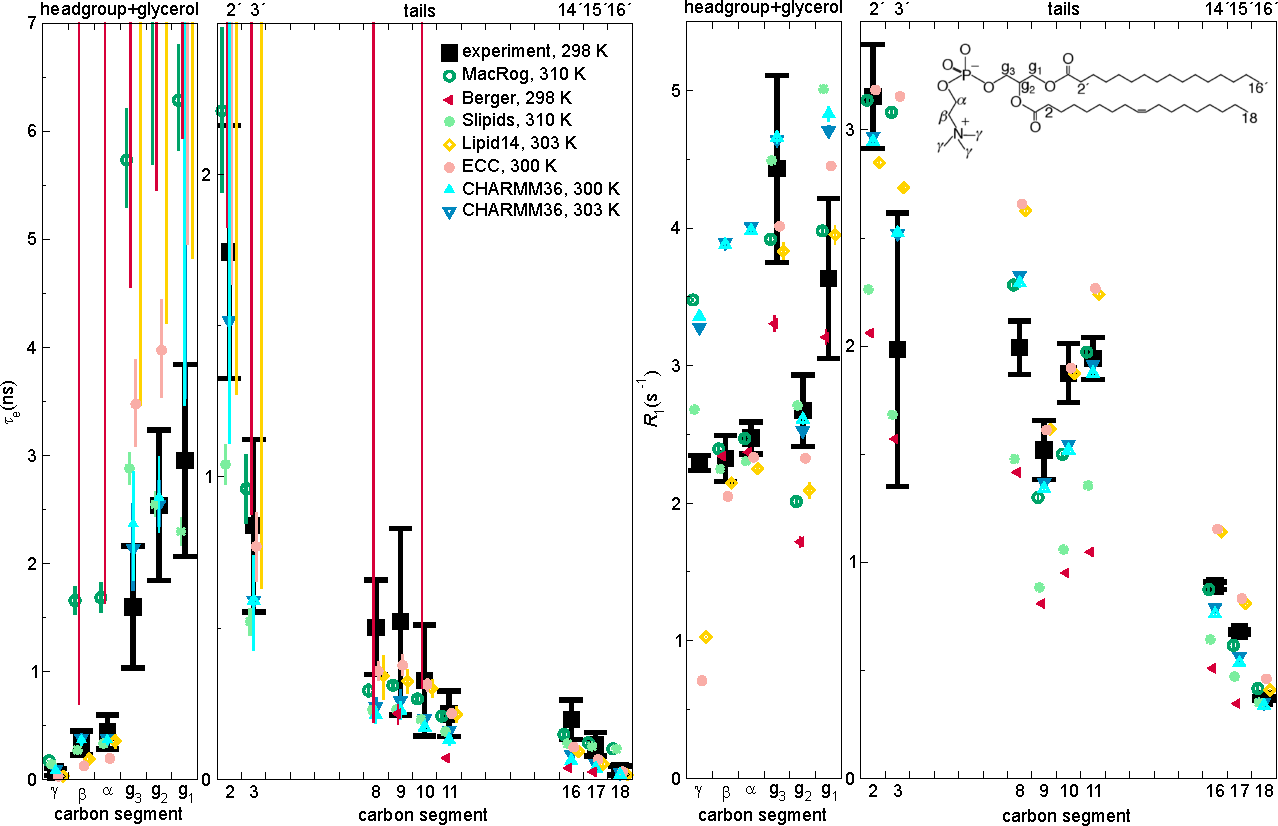
\includegraphics[width=\textwidth]{./figures/normalcond_2020_3.pdf}
\caption{Effective correlation times ($\tau_\mathrm{e}$, left panels) and $R_{1}$ rates (right panels) in experiments (black) and MD simulations (colored) of POPC bilayers in $L_{\alpha}$ phase under full hydration.
Inset on the right shows the POPC structure and carbon segment labeling.
Each plotted value contains contributions from all the hydrogens within its carbon segment; the data for segments 8--11 are only from the sn-2 (oleoyl) chain, whereas the (experimentally non-resolved) contributions of both tails are included for segments 2--3 (2'--3' in the sn-1 chain) and 16--18 (14'--16').
%
Simulation data are only shown for the segments for which there exists experimental data.
%
For $\tau_\mathrm{e}$,
a simulation data point indicates the average over C--H bonds; however,
if $\tau_\mathrm{e}$ could not be determined for all bonds, only the error bar
(extending from the mean of the lower to the mean of the upper error estimates) is shown.
%
The Berger data for methyl segments ($\gamma$, C18, and C16') are left out, because the protonation algorithm used to construct the hydrogens post-simulation in united atom models does not preserve the methyl C--H bond dynamics.
%
Table~\ref{tab:standr} provides further simulation details.
%
Error bars for the experimental values reflect error estimate of {\color{red}XXX}.
}
\label{fig:teff_R1}

\todo{Experimental error estimate changed since the data were originally published; needs to be explained to the reader.}\\
\todo{How to refer to the experiments? Not really from previous publication because of re-analysis.}

\end{figure*}

\subsection*{$R_1$ rates at standard conditions.}
The panels on the right side of Fig.~\ref{fig:teff_R1} compare experimental and simulated $R_{1}$ rates under the same conditions as for the $\tau_\mathrm{e}$ on the left.

There are certain qualitative features that all force fields predict correctly
(for example that $\mathrm g_2$ has the smallest $R_1$ among the glycerol and C9 among the oleoyl double bond segments),
and certain that they all miss (that $R_1$ rates for the oleoyl segments C8, C10, and C11 are all roughly equal).

Quantitatively,
there are a few cases where both $R_1$ and $\tau_\mathrm{e}$ (almost) match experiments, suggesting (almost) correct rotational dynamics at all relevant time scales.
%
%, and for the .
%
For example, 
%LET'S MENTION ONLY THE VERY GOOD ONES
Slipids performs well at the $\beta$ and $\alpha$ segments;
CHARMM36 for the g$_3$, g$_2$,  C2 and C3;
Lipid14 and ECC for the oleoyl double bond; and
MacRog for the tail end segments.

Notably, there are also instances where the $R_1$ comparison distinctly differs from what is seen for $\tau_\mathrm{e}$: Some models that do very well for $\tau_\mathrm{e}$, do rather poorly for $R_1$. Conversely, a matching $R_{1}$ can be accompanied by a larger-than-experimental $\tau_\mathrm{e}$.
% such as CHARMM36 in the $\gamma$, $\beta$, and $\alpha$ segments.
%Also examples to the contrary are seen: MacRog reproduces $R_{1}$ rates well for the $\beta$, $\alpha$, g$_3$, and g$_1$ segments, although it systematically overestimates their $\tau_\mathrm{e}$.
To appreciate such differences,  recall that in order to capture our experimental $R_1$ rates (measured at 125\,MHz) a force field has to have correct rotational dynamics at the $(2\pi\times125~\mathrm{MHz})^{-1}\approx1$\,ns time scale, whereas
$\tau_\mathrm{e}$ reflects all the sub-$\mu$s time scales (Fig.~\ref{fig:schem_teff}).

MacRog for the $\beta$, $\alpha$, g$_3$, and g$_1$ segments provides a prominent example where
the $R_1$ rates are well reproduced, but $\tau_\mathrm e$ times systematically overestimated.
Such a combination suggests that MD does well at the 1\,ns scale, but has too slow long-time dynamics.

The opposite---where $\tau_\mathrm{e}$ matches experiments, but $R_1$ does not---is demonstrated by all five all-atom force fields for the $\gamma$ segment,
%for Slipids around the double bond,
and by CHARMM36 for $\beta$ and $\alpha$. Therein a cancellation of error occurs in $\tau_\mathrm{e}$: The wrong dynamics at the 1\,ns scale are compensated by wrong dynamics at the other time scales.
As CHARMM36 overall performs rather well for both $R_1$ and $\tau_\mathrm{e}$,
we proceed to study this shortcoming on the headgroup $R_1$ rates
in some more detail.
%
%Berger and Slipids for tail segment 2.

%In the tail region, the MD models are in somewhat worse agreement with $R_{1}$ rates than what was seen for $\tau_\mathrm{e}$.
%General tendency for MD to succeed in shorter time scales whereas rotations with slower dynamics are not depicted as well?

\subsection*{Dynamics of headgroup segments in CHARMM36.}

Figure~\ref{fig:cumulativeR1s}A zooms in on the headgroup ($\gamma$, $\beta$, $\alpha$) segments,
whose $\tau_\mathrm e$ were not clearly visible on the scale of Fig.~\ref{fig:teff_R1}.
%
For all three, CHARMM36 matches the experimental $\tau_\mathrm e$,
but overestimates $R_1$.
%
No other force field does any better for $\gamma$, but
for $\beta$ and $\alpha$ Slipids provides almost perfect dynamics.

\begin{figure}[!h]
\centering
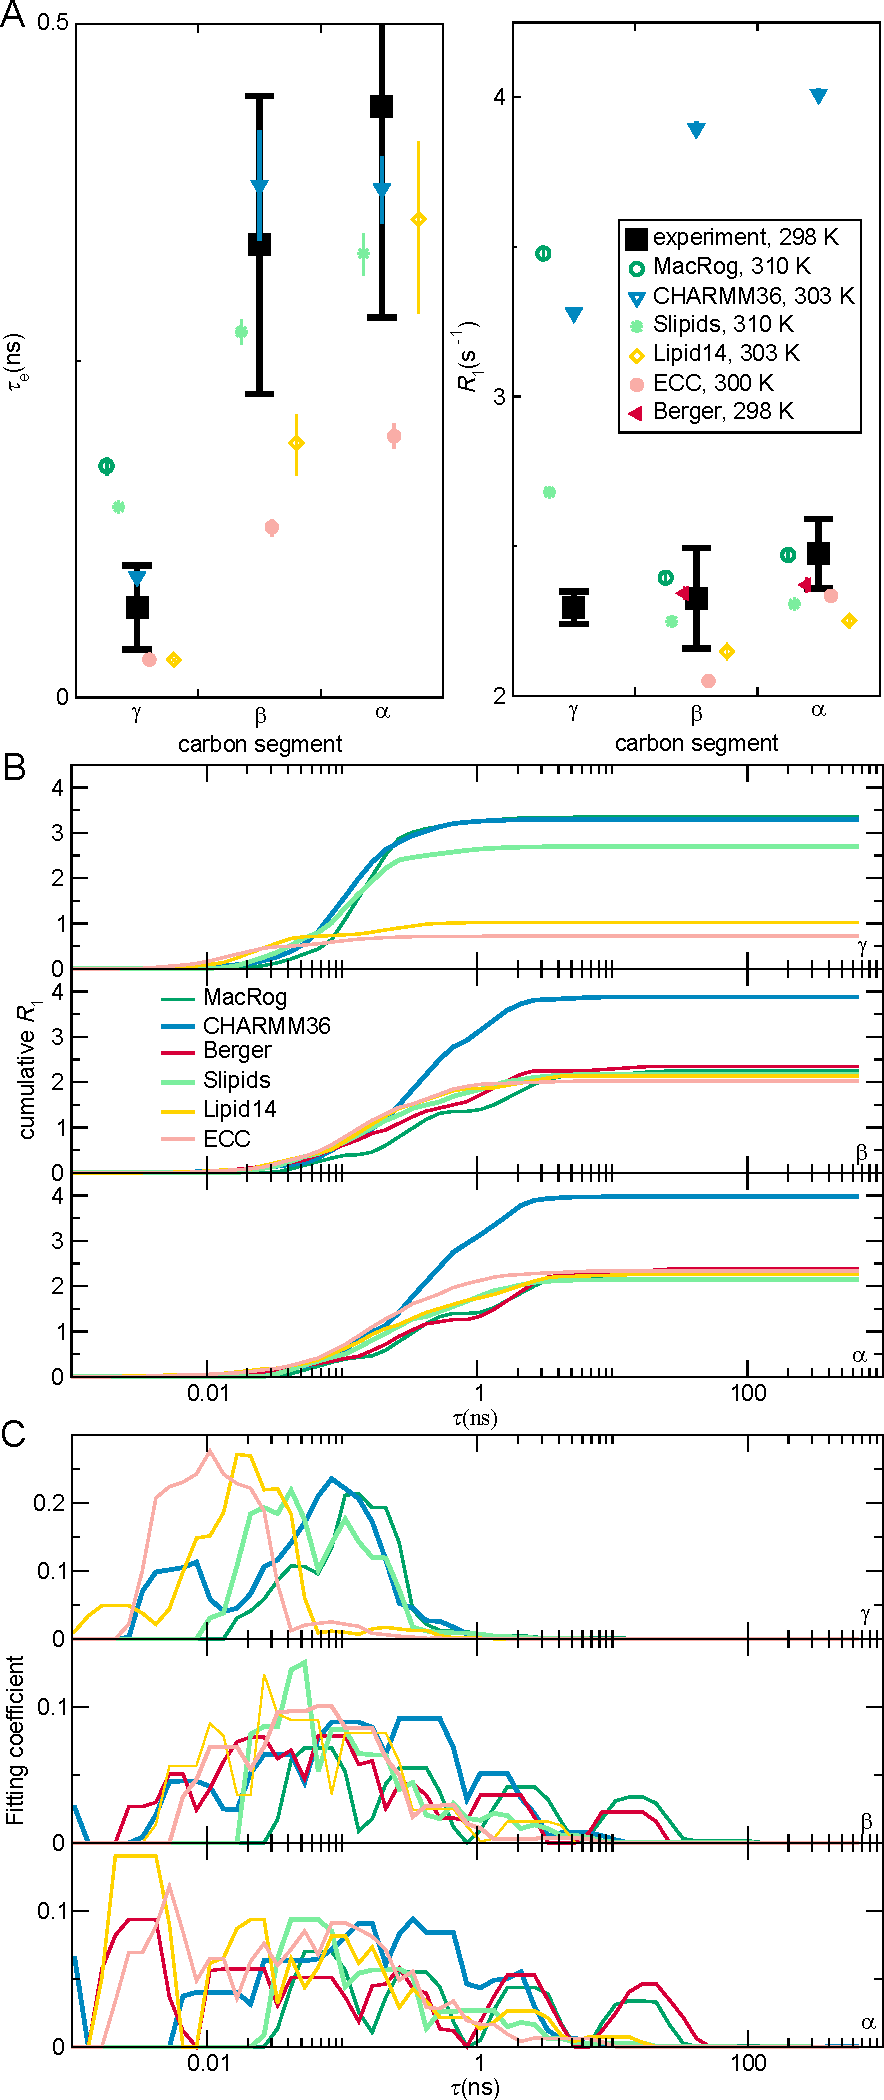
\includegraphics[width=\columnwidth]{../Figs/R1_and_comp.pdf}
\caption{
(A) Zoom on the headgroup $\tau_\mathrm e$ (left panel) and $R_1$ (right).
(B) 'Cumulative' $R_1$ (see Methods for definition) of the
$\gamma$ (top panel), $\beta$ (middle), and $\alpha$ (bottom) segments.
(C) Prefactor weighs $\alpha_i$ from Eq.~\eqref{eq:weights} of $\gamma$ (top), $\beta$ (middle), and $\alpha$ (bottom).
In B and C, a sliding average over 5 neighboring data points is shown.
}
\label{fig:cumulativeR1s}
\end{figure}

To investigate where the differences between force fields arise, we visualize the 
'cumulative' $R_1(\tau)$ in Fig.~\ref{fig:cumulativeR1s}B.
It is obtained, as detailed in Methods,
by including in the sum of Eq.~\eqref{eq:j} only terms with $\tau_i<\tau$.
Consequently, at $\tau\to\infty$ the 'cumulative' $R_1(\tau)$ approaches the actual $R_1$. Ranges of steepest increase therefore indicate time scales that most strongly contribute to $R_1$ rates.

Figure~\ref{fig:cumulativeR1s}B shows
that for models that overestimate the $R_1$ rate of $\gamma$
(MacRog, CHARMM36, and Slipids, see Fig.~\ref{fig:cumulativeR1s}A)
the major contribution to $R_1$ arises at $\tau>50$\,ps, whereas those underestimating the $R_1$ 
(Lipid14 and ECC, see Fig.~\ref{fig:teff_R1})
the major contribution comes from $\tau<50$\,ps. 
%
This also manifests in the
distribution of fitting weights ($\alpha_i$ in Eq.~\eqref{eq:weights}) in Fig.~\ref{fig:cumulativeR1s}C:
The earlier the non-zero weights occur, the smaller is the resulting $R_1$.


For the $\beta$ and $\alpha$ segments, Fig.~\ref{fig:cumulativeR1s}B shows
that the main contribution to $R_1$ rates arises from processes
between 200~ps and 2~ns.
%
As CHARMM36 has the largest weights of all models in this window (Fig.~\ref{fig:cumulativeR1s}C),
it overestimates $R_1$.
%
%For example
In contrast, Slipids, which has simultaneously $R_1$ and $\tau_\mathrm e$ correct,
has its largest weights at $\tau<200$\,ps.
%
Indeed, considerable weights
at short time scales ($<10$\,ps in $\alpha$ for Lipid14, ECC, Berger) and
at long time scales ($>10$\,ns in both $\beta$ and $\alpha$ for MacRog and Berger)
do not manifest at all in the $R_1$ rates.
%
However, the latter contribute heavily on $\tau_\mathrm e$,
which is thus considerably overestimated by MacRog and Berger (Fig.~\ref{fig:teff_R1}).

What are the motions in the 0.2--2\,ns window that are over-presented in CHARMM36?
Identifying them and speeding them up would improve the model dynamics.
However, the connection between the fitted correlation times and the correlation times of distinct motional processes, such as dihedral rotations and lipid wobbling, turns out to be highly non-trivial; we thus refrain from further analysis here.

\subsection*{Effect of cholesterol.}
The experimental effective correlation times $\tau_\mathrm e$
(Fig.~\ref{fig:chol}A, top panels)
show that when cholesterol is added,
the glycerol region conformational dynamics
slow down markedly.
%
The tail segments slow down too,
the effect increasing towards the backbone.

In stark contrast, however,
the $\tau_\mathrm e$ of headgroup segments ($\gamma$, $\beta$, $\alpha$)
are unaffected by cholesterol.
%
Furthermore, cholesterol induces no measurable change in the
headgroup $\beta$ and $\alpha$ segment
dynamics at short ($\sim$1\,ns) time scales, as
demonstrated by
the experimental $R_{1}$ rates (Fig.~\ref{fig:chol}A, lower panels).
That said,
there is a small but measurable impact on $R_1$ at $\gamma$.

All the force fields investigated qualitatively reproduce the increase in $\tau_\mathrm e$ (see Fig.~\ref{fig:chol}B):
Slipids gives the best magnitude estimates, while CHARMM36 and MacRog clearly overestimate the changes at the glycerol, C2, and C3 carbons. Notably, MacRog \todo{and Berger?} erroneously predict slow down also for the $\beta$ and $\alpha$ carbons, for which experiments detect no change.
%
Note that,  while CHARMM36 correctly shows no chance in $\tau_\mathrm{e}$
of the $\gamma$, $\beta$, and $\alpha$ carbons,
it predicts a non-zero $\Delta R_{1}$ for all three, indicating some inaccuracies in the
headgroup rotational dynamics. % at shorter time-scales.
Such inaccuracies might be reflected in the recent findings~\cite{leeb18}
(obtained using CHARMM36)
that 
%(at least at small cholesterol concentrations)
the headgroups of PCs neighbouring a cholesterol (within 6.6\,\AA) spend more time on top of the cholesterol than elsewhere;
such arrested rotations could manifest on $\tau_\mathrm e$ and $R_1$.
%
Interestingly, 
the tail $\Delta R_{1}$ seem to be pretty well reproduced by
all three all-atom force fields, whereas Berger fails to capture the change at the oleoyl double bond.

%Along with the slow-down of dynamics, all the models show an increase in the $\vert S_{\rm{CH}}\vert$ upon addition of cholesterol at the tail region (\todo{Show data?}), reflecting the reduced available volume for the POPC.\todo{Is this a known effect/explanation?}

%The change observed here, however, is particularly sensitive to the length of the trajectory as cholesterol-induced increase in effective correlation time is likely to lead to worse convergence of the correlation function within the limited simulation time, and more drastic underestimation of $\tau_\mathrm{e}$ is expected than for simulations without cholesterol. This will, consequently, cause a tendency towards underestimation on the strength of the cholesterol-driven modulation of the effective correlation time.

\begin{figure}[h!]
	\centering
	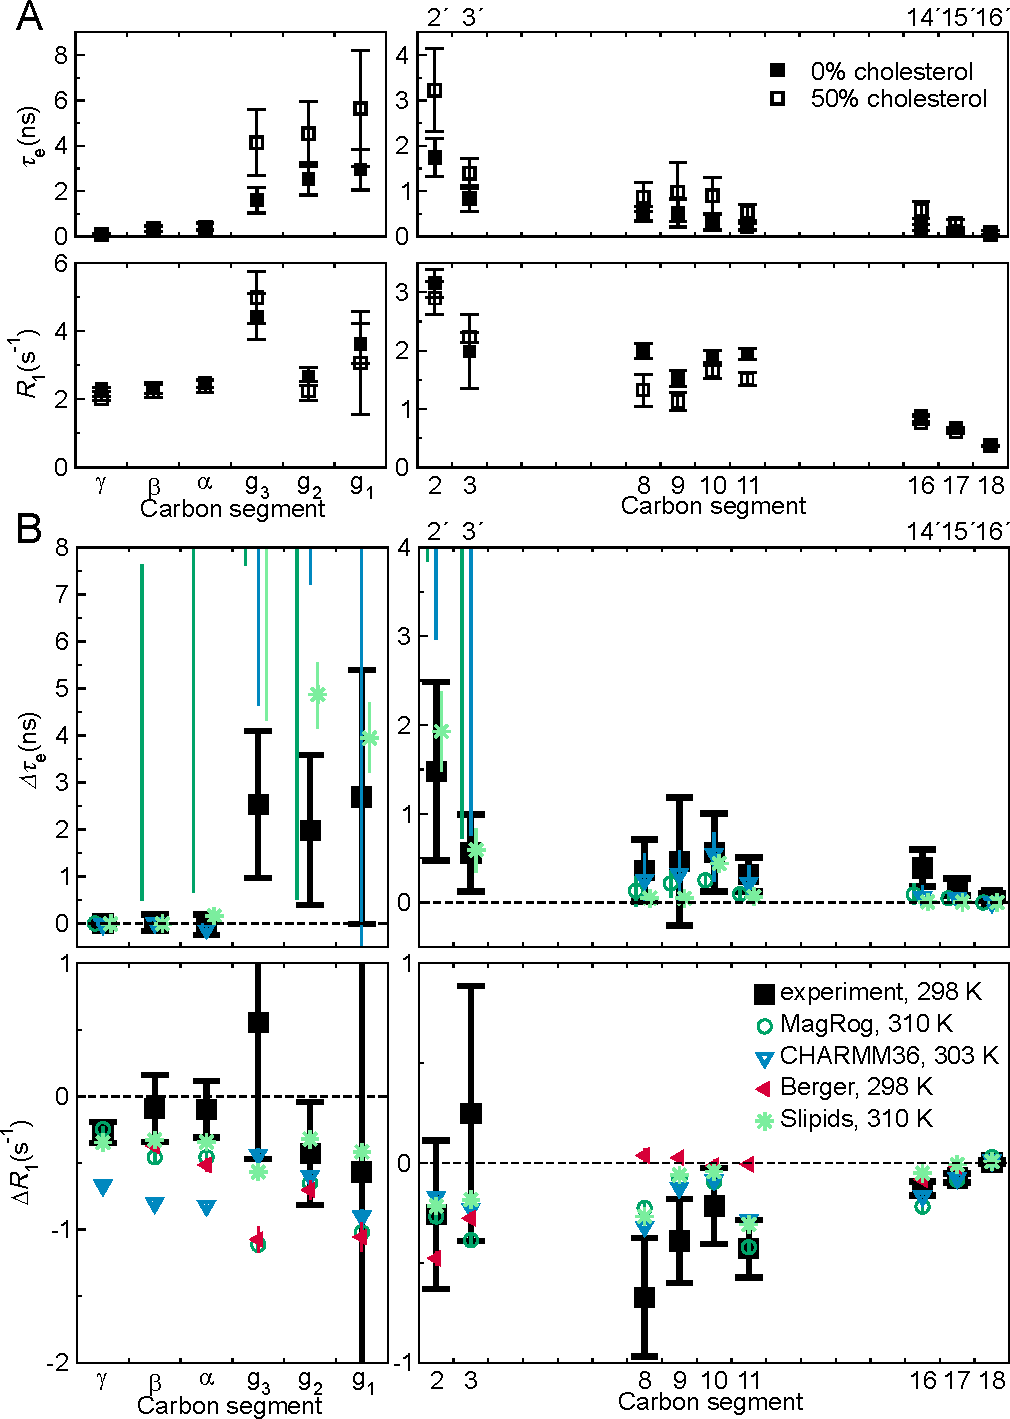
\includegraphics[width=\columnwidth]{./figures/cholesterol.pdf}  
	\caption{Effect of bilayer cholesterol content.
	(A) The experimental effective correlation times $\tau_\mathrm{e}$ (top panels) and $R_{1}$ rates (bottom) in a pure POPC bilayer and in a bilayer containing 50\% cholesterol. The data were measured at 298\,K and full hydration.
	(B) The change in $\tau_\mathrm{e}$ ($\Delta\tau_\mathrm{e}$, top panels) and $R_{1}$ ($\Delta R_{1}$, bottom),
	both in experiments and in MD simulations, when bilayer composition changes from pure POPC to 50\% cholesterol.
	Berger not shown for $\Delta\tau_\mathrm{e}$, because the open data available were insufficient to determine meaningful error estimates.
	Error estimates for the simulated $\Delta\tau_\mathrm e$ are the maximal possible
	based on the errors at 0\% and 50\% cholesterol;
	for other data regular error propagation is used.
	Table~\ref{tab:chol} provides further simulation details;
	for segment labeling, see Fig.~\ref{fig:teff_R1}.
	}
	\label{fig:chol}
\todo{@Hanne: Double check that the calculation of errors in (B) was as the caption describes.}
\todo{Check if cholesterol data is in full hydration}
\end{figure}


\subsection*{Effect of drying.}
Figure~\ref{fig:hydration}A shows how a mild dehydration affects
C--H bond dynamics in the PC headgroup and glycerol backbone;
the plot compares the experimental effective correlation times $\tau_\mathrm e$
measured for POPC at full hydration and for DMPC (1,2-dimyristoyl-sn-glycero-3-phosphocholine)
at 13 waters per lipid.


The $\tau_\mathrm e$ are the same within experimental accuracy, which suggests two conclusions. Firstly, 
the headgroup ($\gamma$, $\beta$, $\alpha$) $\tau_\mathrm e$ are unaffected by structural differences in the tails. This is analogous to  what was seen experimentally when adding cholesterol
(Fig.~\ref{fig:chol}): Changes in the tail and glycerol regions do not reflect to the headgroup. Secondly, a mild dehydration does not alter the $\tau_\mathrm e$
in the headgroup and glycerol regions. 

\begin{figure}[ht!]
\centering
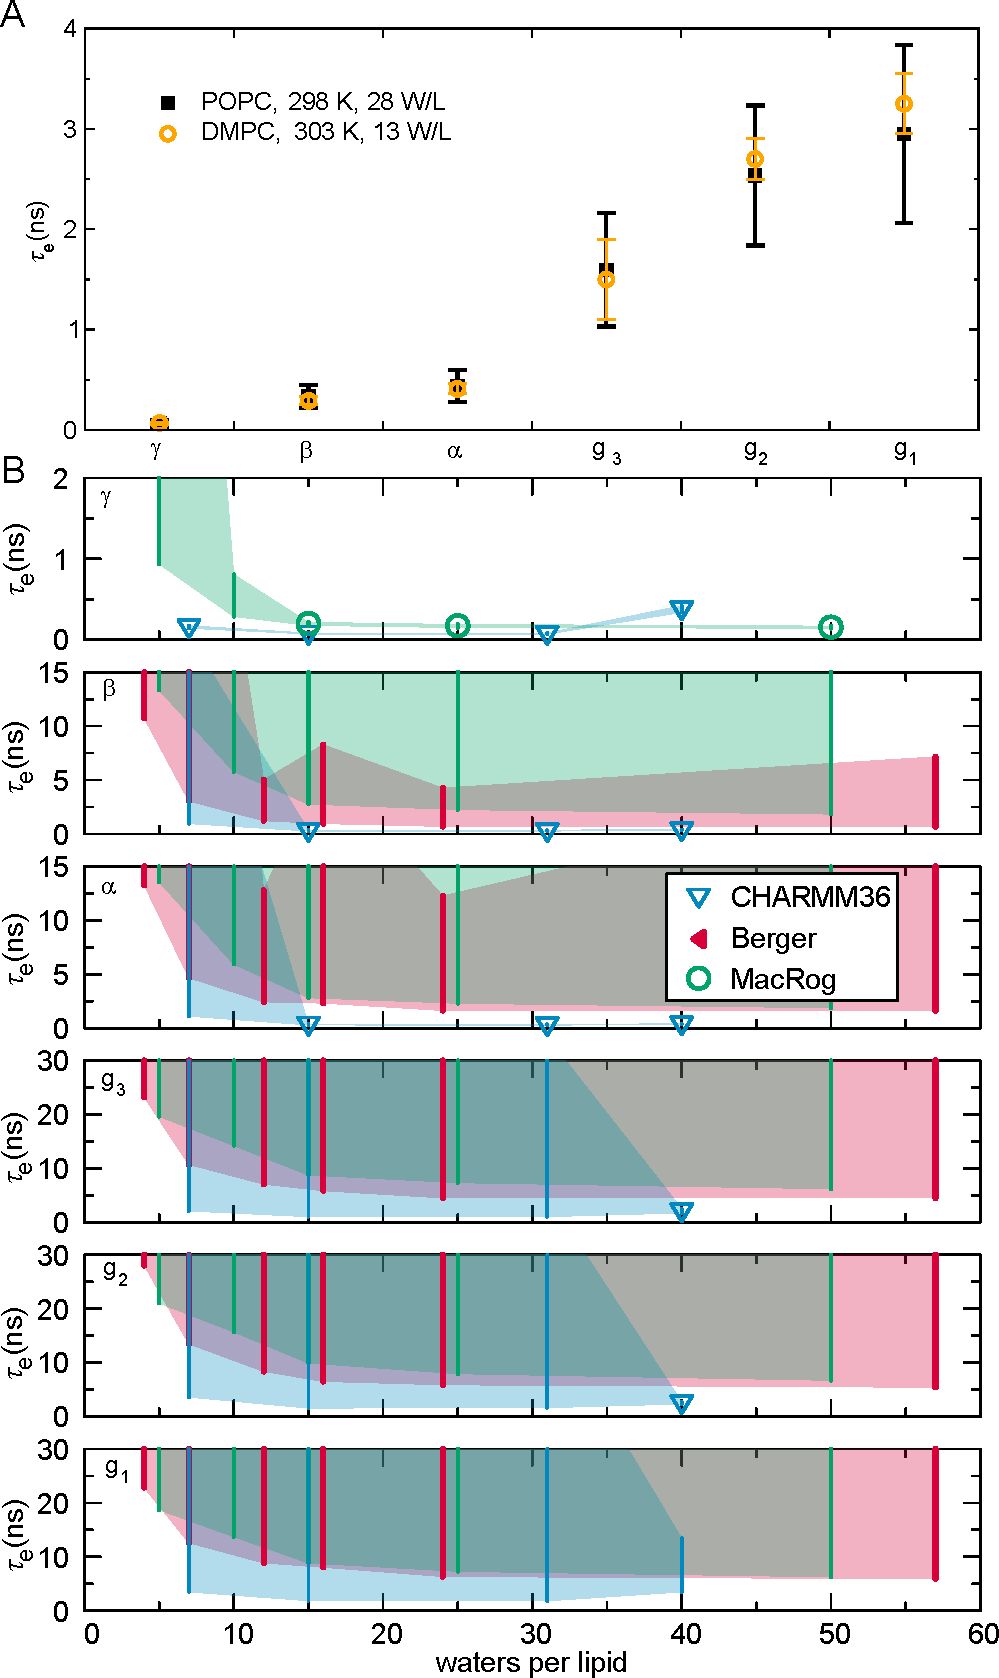
\includegraphics[width=\columnwidth]{../Figs/hydration_2020.pdf} 

\subsection*{Effect of dehydration.}
The impact of dehydration on the structure and dynamics of lipid bilayers is of considerable interest as  membrane fusion is always preceeded by removal of water between the opposing membranes and therefore may affect the rate of fusion. Lipid bilayers in dehydrated states are also found, e.g., in skin tissue. 

Figure~\ref{fig:hydration}A shows how a mild dehydration affects
C--H bond dynamics in the PC headgroup and glycerol backbone;
the plot compares the experimental effective correlation times $\tau_\mathrm e$
measured for POPC at full hydration and for DMPC (1,2-dimyristoyl-sn-glycero-3-phosphocholine)
at 13 waters per lipid.


The $\tau_\mathrm e$ are the same within experimental accuracy, which suggests two conclusions. Firstly, 
the headgroup ($\gamma$, $\beta$, $\alpha$) $\tau_\mathrm e$ are unaffected by structural differences in the tails. This is analogous to  what was seen experimentally when adding cholesterol
(Fig.~\ref{fig:chol}): Changes in the tail and glycerol regions do not reflect to the headgroup. Secondly, a mild dehydration does not alter the $\tau_\mathrm e$
in the headgroup and glycerol regions. 

\begin{figure}[ht!]
\centering
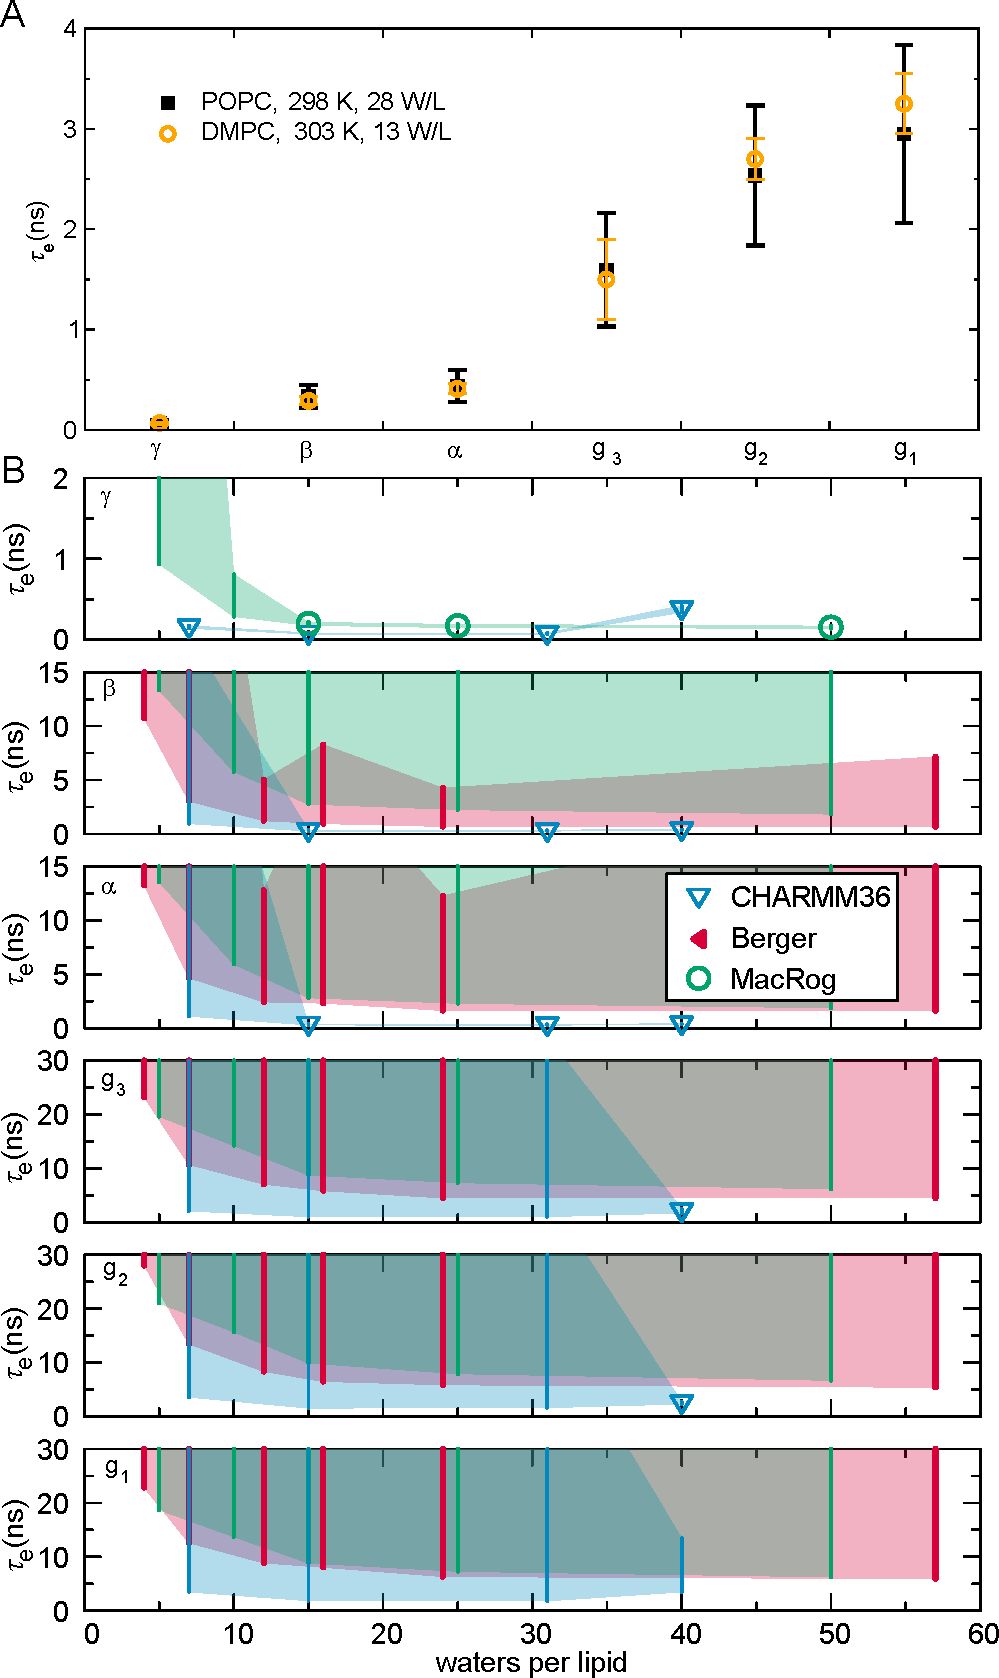
\includegraphics[width=\columnwidth]{../Figs/hydration_2020.pdf} 

\caption{Effect of drying on %the
effective correlation times %$\tau_\mathrm e$
in headgroup and glyc\-er\-ol backbone.
(A) Experimental $\tau_\mathrm e$ for
DMPC (from Ref.~\citenum{pham15}) at low hydration %(13\,w/l)
do not significantly differ from the
$\tau_\mathrm e$ for POPC at full hydration. %(28\,w/l)
(B) Calculated $\tau_\mathrm e$  for
POPC at decreasing hydration in three MD models.
Note that three Berger data points (4, 12, 16, and 24~w/l) are from DLPC bilayers.
Symbols give the mean of segment hydrogens,
if $\tau_\mathrm{e}$ could be determined for all hydrogens; else only the error bar
(extending from the mean of the lower to the mean of the upper uncertainty estimates) is shown;
the area delimited by the error bars is shaded for visualization.
See Table~\ref{tab:hydr} for simulation details.}
\label{fig:hydration}
\todo{How to refer to full hydration POPC data?}\\
\end{figure}

Figure~\ref{fig:hydration}B shows the effects of dehydration in three MD models.
Combination of
the unrealistically slow dynamics, especially in the glycerol backbone, (Fig.~\ref{fig:teff_R1}) and
the relatively short lengths of the openly available trajectories %with dehydration conditions
(Table~\ref{tab:hydr})
led to large uncertainty estimates. %for simulation data are large. %which makes discussion challenging.
%

Owing to the uncertainties, we only point out the qualitative trends. For all carbons in the headgroup and glycerol segments, the simulated  $\tau_\mathrm e$ indicates slow down upon dehydration. This is manifested in the increase in the magnitude of the error estimate (cf. the Berger data for $\beta$ and $\alpha$) as well as in the increase of the lower limit of the error. 
For CHARMM36 the lower error estimates almost constant all the way until 7\,w/l, whereas for Berger and MacRog they indicate a retardation of the dynamics starting already from $\sim$20\,w/l.

These simulational findings suggest that
experiments reducing hydration levels below 10\,w/l would also show an increase in $\tau_\mathrm e$.
This prediction is in line with the
exponential slow-down
%(decay constant $\sim$4 removed waters per lipid)
of the headgroup conformational dynamics
upon dehydration that was indicated by $^2$H-NMR $R_{1}$ measurements
of DOPC bilayers:
$R_1\sim\exp(-n_{{\mathrm w\!}_{/\mathrm l}}/4)$~\cite{ulrich94}.
%
The slowdown was attributed to the reduction in the effective volume available for the headgroup~\cite{ulrich94}
owing to its tilt towards the membrane upon dehydration;
the tilt is observed via changes of the lipid headgroup order parameters~\cite{bechinger91},
and is qualitatively reproduced by all the simulation models~\cite{botan15}.

%{\color{red} Cite also the D$_2$O data. \cite{Volke:1994b}}
%{\color{blue} There are also data for the tails. \cite{Volke:1982a}}
%{\color{green} Ref.~\citenum{Faure:1997a}: Each DMPC in fluid phase binds $\sim$10 D$_2$O.}


Figure~\ref{fig:hydration}C shows
a collection of experimental $^{13}$C-NMR $R_1$ rates
measured at 125\,MHz for the headgroup segments
at different water contents;
in addition to the full hydration POPC data from Fig.~\ref{fig:teff_R1},
DMPC at 13\,w/l~\cite{pham15}, % 125 MHz, 300K
and POPC at 20 and 5\,w/l~\cite{Volke:1995a} %125.76 MHz, 298K
are shown.
%
An increasing trend with decreasing hydration is observed for all the segments,
indicating changes of headgroup dynamics at short ($\sim$1\,ns) time scales.
Interestingly, only CHARMM36 captures this,
whereas Berger and MacRog give decreasing $R_1$ rates for $\beta$ and $\alpha$.
%
\begin{figure}[ht!]
\centering
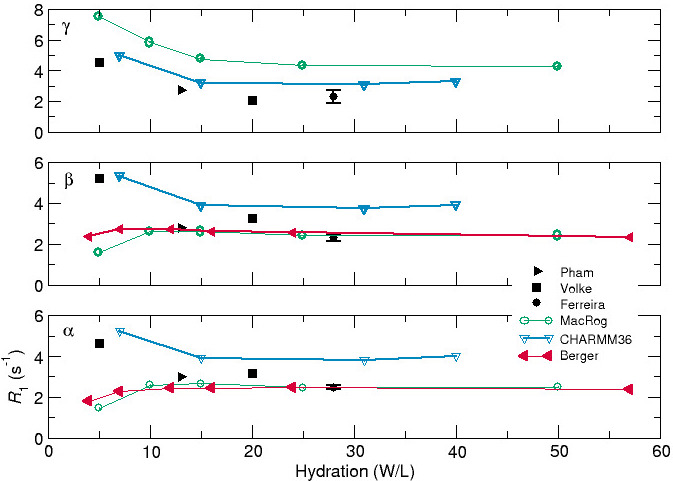
\includegraphics[width=\columnwidth]{../Figs/dehydrationR1.jpeg} 
\caption{Effect of drying on $^{13}$C-NMR $R_1$ rates of the headgroup segments (at 125\,MHz)
in experiments and simulations.}
\label{fig:dehydrationR1}
\todo{HA:  merge this with the Fig.~\ref{fig:hydration}}
\end{figure}

The characteristics of the slow down discussed here are of significance
not only for computational studies of inter\-membrane interactions, such as membrane fusion,  but also when simulating a bilayer (stack) under low hydration. Slower dynamics imply that longer simulation times are needed for equilibration, for reliably quantifying the properties of the bilayers, and for observing rare events. %such as the lipid tail flips from one membrane to another in case of the fusion~\cite{best citation here}. Same applies in simulations performed in increasing concentrations of cholesterol, as the slow down of dynamics and the increase of tail order parameters observed therein are analogous to those occurring upon dehydration. \todo{really not the smoothest text}
%Sims by Calero~\cite{Calero:2019a} for water dynamics at membrane


\subsection*{Effect of cation binding.}
\todo{This section will (possibly) be on ECC simulations and how teff chances with (divalent?) ion binding}

Finally, we comment on the response of the MD model dynamics to increasing amounts of salt.
%To our knowledge, no experimental $^{13}$C-NMR $R_1$ or $\tau_\mathrm e$ data exists as a function of monovalent salt concentration; therefore, the following discussion is kept qualitative.
Experimentally, the modulation of $\alpha$ and $\beta$ carbon order parameters upon increasing ion concentration have been used to quantify ion binding to lipid bilayers (the molecular electrometer~\cite{seeling87,catte16}). The order parameters are constant for POPC bilayers under NaCl addition in experiments, indicating negligible ion binding, but change in the presence increasing amounts of divalent ions. %Based on this, we anticipate the effective correlation times also to be unaffected by monovalent salt. %however, to our knowledge no experimental measurements have been conducted to quantify this.

The molecular electrometer has been used to show that most molecular dynamics force fields overestimate the binding of monovalent ions to PC bilayers~\cite{catte16}: In the simulations the modulation of the $\alpha$ and $\beta$ carbon order parameters by increasing NaCl concentration was overestimated compared to the experiments, and accompanied by accumulation of ions at the bilayer surface. Here, we use existing data from a force field, the ECC model, that is know to have mostly realistic ion binding. 


This indicates that, similarly to the order parameters, $\tau_{\rm{e}}$ may be useful in investigating the ion binding affinity of lipid bilayers and experimental work exploring this avenue would be interesting.   


\begin{figure}[ht!]
\centering
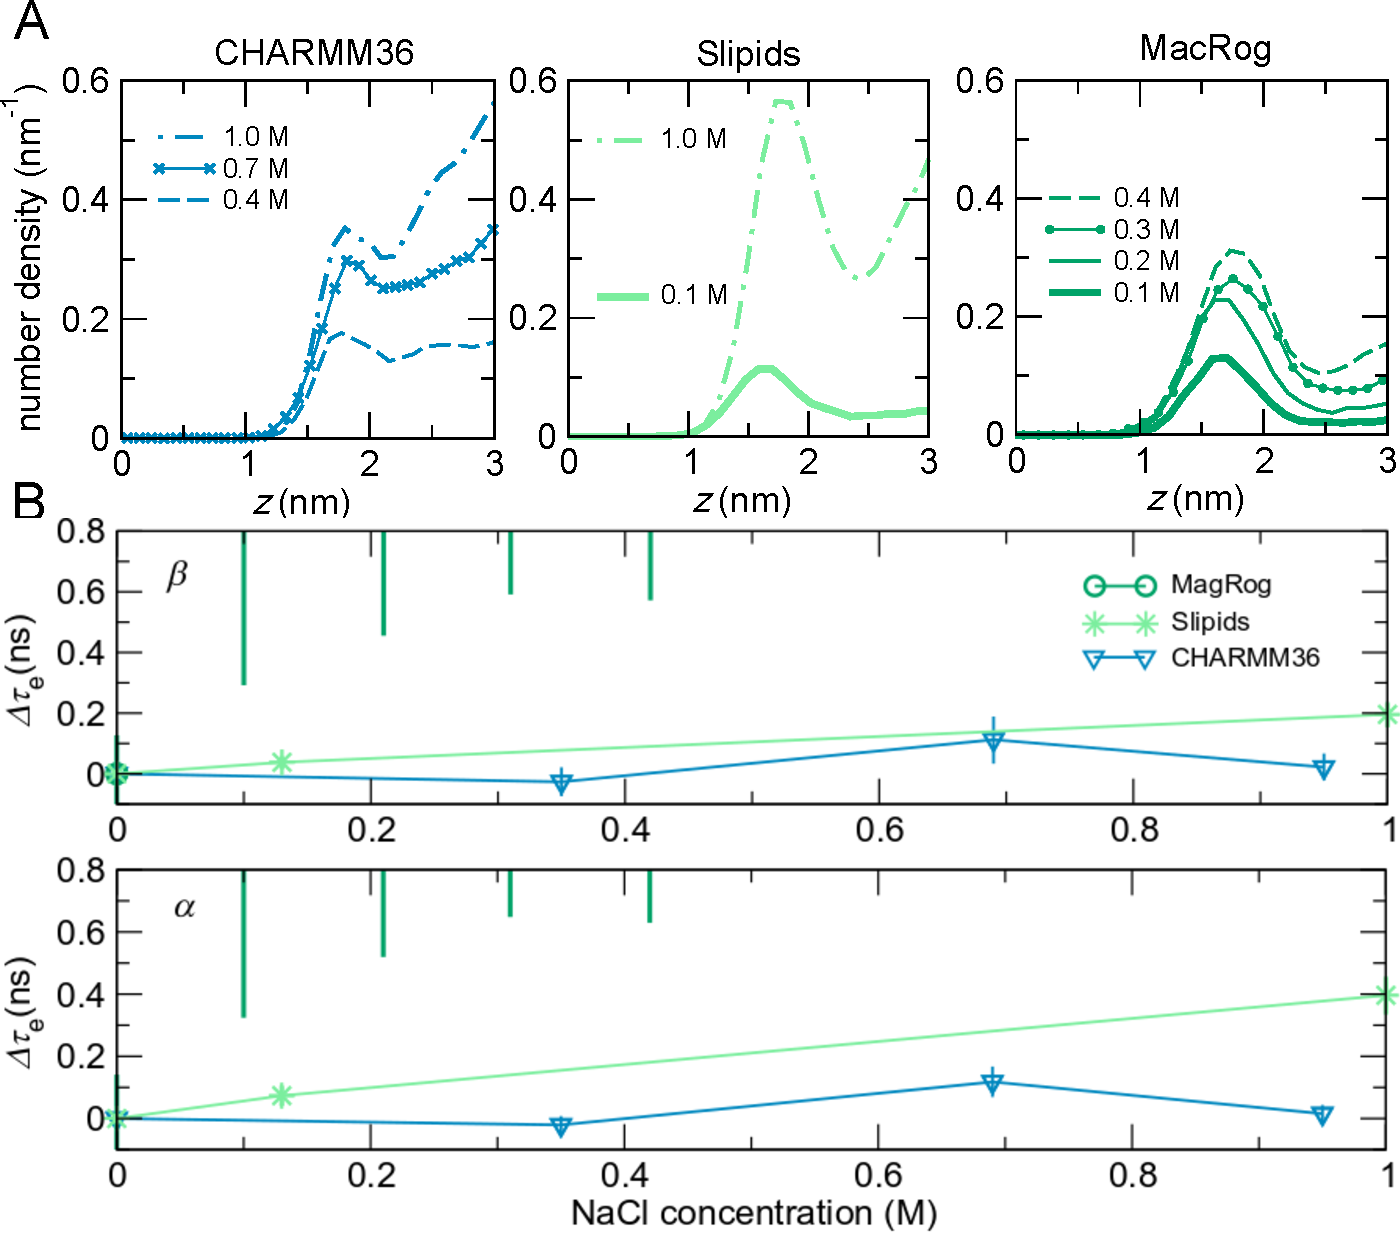
\includegraphics[scale=0.36]{./figures/salt.pdf} 
\caption{A picture of alpha and beta teff vs bound CA ions in the ECC model}
\label{fig:salt}
\todo{analysis running}
\end{figure}

\section{Conclusions}

\section{Conclusions}
Open access databanks of MD trajectories enables the creation new scientific information without running a single new simulation. Here,
we demonstrated this by investigating the dynamics of a wide range of phosphatidylcholine molecular dynamics models using the existing trajectories from the NMRlipids databank.

We found that MD qualitatively captures the $^{13}$C-NMR effective correlation time ($\tau_\mathrm e$) profile of POPC---the slow glycerol backbone and the faster motions of the headgroup and tail regions---but most MD force fields are prone to too slow dynamics of the glycerol C--H bonds (Fig.~\ref{fig:teff_R1}).
%
While no force field reproduces all the experimental data,
CHARMM36 and Slipids have an overall impressive $\tau_\mathrm e$.
This is particularly true for CHARMM36, as it is also known to
well reproduce the experimental conformational ensemble~\cite{botan15}.
%
That said, we find that CHARMM36 struggles with the balance of dynamics in the headgroup region:
The $R_1$ rates, sensitive for $\sim$1-ns processes, are too high for the $\gamma$, $\beta$, and $\alpha$ segments (Fig.~\ref{fig:cumulativeR1s}).

\todo{Make the point that the 500-ns simulations indicated by Vogel~\cite{vogel12} are not needed for sufficient sampling?}

In addition to standard conditions, we explored how the dynamics react to addition of cholesterol or NaCl, or to removal of water.
%
MD qualitatively captures that when cholesterol is mixed into a POPC bilayer, the conformational dynamics in the tail and glycerol regions slows down; however, some force fields predict an (erroneous) slowdown also for the headgroup (Fig.~\ref{fig:chol}).
%
With increasing NaCl concentration, a behaviour reminiscent of the molecular electrometer was observed: Amount of ion binding to the bilayer correlated with the magnitude increase in $\tau_\mathrm e$; this could open up the possibility of using $\tau_\mathrm e$ in quantifying cation binding to lipid bilayers.
%
When reducing the water content, MD exhibits slowdown of headgroup and backbone dynamics below $\sim$10 waters per lipid in qualitative agreement with experimental data. \todo{ Hydration needs some kind of statement of significance.}

By gathering a set of $^{13}$C-NMR data on the phosphatidylcholine dynamics and charting the typical features of the existing MD models against it, this study lays the foundation for further improvement of the force fields. While work is still needed in capturing even the correct conformations~\cite{botan15}, realistic dynamics will be an essential part of developing MD into a true computational microscope.

Importantly, this work demonstrates the power of open data in creating new knowledge out of existing trajectories at a reduced computational and labor cost. %Although no new simulations were performed for the purpose of this work, we were able to conduct a comprehensive study on the dynamics of MD models under several conditions. An interesting extension would be exploring other lipid headgroups individually as well as performing a comparison of MD model dynamics between headgroup types, as the available simulation data goes well beyond simulations of lipids with the phosphocholine headgroup.
If the data are well indexed and documented, this process could be automated and has the potential to facilitate faster progress, e.g., in the development of MD force fields, for example through machine learning approaches.


\acknowledgement
  This material is based upon work supported by XXX under Grant No. XXX. The project is/isn't part of the NMRlipids open collaboration (nmrlipids.blogspot.fi)

\bibliography{lipids,ff,simu,pdb,journals}

\begin{tocentry}
 % \includegraphics[width=77mm]{abstract_figure}
 TOC here if needed
\end{tocentry}

\end{document}
